

\documentclass[10pt,a4paper]{report}
\usepackage[utf8]{inputenc}
\usepackage[english]{babel}
\usepackage{amsmath}
\usepackage{amsfonts}
\usepackage{amssymb}
\usepackage{graphicx}
\usepackage{caption}
\usepackage{float}
\usepackage{array} 
\usepackage{booktabs}	% for horizontal lines
\usepackage{varwidth}% http://ctan.org/pkg/varwidth
\usepackage{csvsimple} % automatic table generation from csv files
\usepackage{comment}
\usepackage[style=draft, backend=bibtex]{biblatex}

% Macros zum Setzen von Formeln
%-------------------------------

\newcommand{\gradient}[1]{\left(\nabla #1 \right)}
\newcommand{\hesse}[1]{\left(\nabla^2 #1 \right)}
 
% transponiert
\newcommand{\transpose}[1]{#1^\mathrm{T}}
% Exponentialfunktion
\newcommand{\e}{\mathrm{e}}
% Imagin�re Einheit
\newcommand{\I}{\mathrm{I}}
% Einheitsmatrix E
\newcommand{\II}{\vec{E}} 
% Ableitungen
\newcommand{\dd}{\mathop{}\!\mathrm{d}}
\newcommand{\Diff}[2]{\frac{\dd#1}{\dd#2}}
\newcommand{\DiffT}[1]{\Diff{}{t}#1}
\newcommand{\DDiff}[2]{\frac{\dd^2}{\dd#2^2}#1}
\newcommand{\DDiffT}[1]{\DDiff{#1}{t}}
\newcommand{\PartDiff}[2]{\frac{\partial #1}{\partial #2}}
\newcommand{\PartDiffT}[1]{\Diff{#1}{t}}
\newcommand{\PartDDiff}[2]{\frac{\partial^2 #1}{\partial #2^2}}
\newcommand{\PartDDiffT}[1]{\DDiff{#1}{t}}

\newcommand{\lie}[1]{\mathrm{L}_{#1}}
\newcommand{\ad}[1]{\mathrm{ad}_{#1}}

% Betrag und Norm
\newcommand{\abs}[1]{\mleft\vert#1\mright\vert}
\newcommand{\norm}[1]{\mleft\Vert#1\mright\Vert}

% Macro f�r die Abst�nde in Gleichungen mit Nebenbedingungen
\providecommand{\with}{\,, & \qquad}
% Satzzeichen nach Formeln
\providecommand{\FullStop}{\text{~\@.\xspace}}
\providecommand{\Comma}{\text{~,\xspace}}

% Klammern
\providecommand{\of}[1]{\mleft(#1\mright)}
\newcommand{\braces}[1]{\mleft(#1\mright)}
\newcommand{\set}[1]{\mleft\{#1\mright\}}

% Variante f�r \left. und \right\. ohne Abstand
\providecommand{\mleftdot}{\mleft.\kern-\nulldelimiterspace}
\providecommand{\mrightdot}{\mright.\kern-\nulldelimiterspace}

\let\originalleft\left
\let\originalright\right
\renewcommand{\left}{\mleft}
\renewcommand{\right}{\mright}



% Zahlenmengen
\newcommand{\numset}[1]{\mathbbm{#1}}

\newcommand{\eps}{\varepsilon}

% Operatoren
\DeclareMathOperator{\sign}{sgn}
\DeclareMathOperator{\rang}{rang}
\DeclareMathOperator{\Real}{Re}
\DeclareMathOperator{\Imag}{Im}
\DeclareMathOperator{\grad}{grad}
\DeclareMathOperator{\adj}{adj}
\DeclareMathOperator{\Span}{span}
\DeclareMathOperator{\asin}{asin}
\DeclareMathOperator{\acos}{acos}
\DeclareMathOperator{\atan}{atan}
\DeclareMathOperator{\asinh}{asinh}
\DeclareMathOperator{\acosh}{acosh}
\DeclareMathOperator{\atanh}{atanh}

\newcommand{\diag}{\operatorname*{diag}}
\renewcommand{\ker}{\operatorname*{Kern}}
\newcommand{\bild}{\operatorname*{Bild}}
\newcommand{\konst}{\operatorname*{konst.}}
\newcommand{\const}{\operatorname*{const.}}

% Makro f�r Vektoren (unterscheide griechische Buchstaben)
\DeclareRobustCommand{\vec}[1]{ 				
	\ifthenelse{\equal{#1}{\omega} \OR \equal{#1}{\varphi} \OR \equal{#1}{\alpha} \OR \equal{#1}{\beta} \OR \equal{#1}{\chi} \OR \equal{#1}{\delta} \OR \equal{#1}{\varepsilon} \OR \equal{#1}{\phi} \OR \equal{#1}{\epsilon} \OR \equal{#1}{\gamma} \OR \equal{#1}{\eta} \OR \equal{#1}{\iota} \OR \equal{#1}{\kappa} \OR \equal{#1}{\lambda} \OR \equal{#1}{\mu} \OR \equal{#1}{\nu} \OR \equal{#1}{\pi} \OR \equal{#1}{\theta} \OR \equal{#1}{\vartheta} \OR \equal{#1}{\rho} \OR \equal{#1}{\sigma} \OR \equal{#1}{\varsigma} \OR \equal{#1}{\tau} \OR \equal{#1}{\upsilon} \OR \equal{#1}{\xi} \OR \equal{#1}{\psi} \OR \equal{#1}{\zeta}}{
		% F�r griechische Kleinbuchstaben muss boldsymbol verwendet werden (deckt mathbf nicht ab)
		\boldsymbol{#1}
	}{
		% Alle anderen Symbole verwenden mathbf
		\mathbf{#1}
	}
}


%------------------------------
% Macros zur Verwendung im Text
%------------------------------

% Namen
%-------
\providecommand{\Maple}{\textsc{Maple}\xspace}
\providecommand{\Matlab}{\textsc{Matlab}\xspace}
\providecommand{\MatlabSimulink}{\textsc{Matlab/Simulink}\xspace}
\providecommand{\Doxygen}{\textsc{Doxygen}\xspace}

% +++ English
% .\@ is not treated as a full stop (important for the length of the whitespace
% afterwards. \@. is always treated as a full stop.)
\providecommand{\ie}{i.\,e.\@\xspace} 
\providecommand{\eg}{e.\,g.\@\xspace}
\providecommand{\cf}{cf.\@\xspace}

% +++ German
\providecommand{\zB}{z.\,B.\@\xspace}
\providecommand{\ZB}{Z.\,B.\@\xspace}
\providecommand{\bzw}{bzw.\@\xspace}
\providecommand{\bspw}{bspw.\@\xspace}
\AtEndOfClass{\renewcommand{\dh}{d.\,h.\@\xspace}}
\providecommand{\Dh}{D.\,h.\@\xspace}
\providecommand{\ua}{u.\,a.\@\xspace}
\providecommand{\sog}{sog.\@\xspace}
\providecommand{\usw}{usw.\@\xspace}
\providecommand{\etc}{etc.\@\xspace}
\providecommand{\ggf}{ggf.\@\xspace}
\providecommand{\ca}{ca.\@\xspace}
\providecommand{\uU}{u.\,U.\@\xspace}
\providecommand{\vgl}{vgl.\@\xspace}

% f�r W�rter mit Bindestrich. (Setzt einen Bindestrich, an dem nicht getrennt
% werden darf, l�sst aber die Trennung im folgenden Wort zu.)
\providecommand{\hypII}[2]{#1\nobreakdash-\hspace{0pt}#2}
\providecommand{\x}[1]{\hypII{$x$}{#1}}
\providecommand{\y}[1]{\hypII{$y$}{#1}}
\providecommand{\z}[1]{\hypII{$z$}{#1}}

%--- Zeilenhoehe in Tabellen -------------------------------------------------
% Mit dem Befehl \TabEqn kann eine Formel in einer Tabelle gesetzt werden
% (einfach nur die Formel in die Tabelle eingeben bringt die vertikale
% Ausrichtung irgendwie durcheinander)
% \ExtraTabEqnSpace ist der Platz, der oben und unter einer Formel eingef�gt
% wird
\AtEndOfClass{
\newcommand{\ExtraTabEqnSpace}{1ex}
\makeatletter
\newcommand*{\TabEqn}[1]{%
\begingroup
	\setbox\@tempboxa=\hbox{%
	#1%
	}%
	% Hinzufuegung von 1ex zu Hoehe (\ht)
	% und Tiefe (\dp) der Box.
	% Umweg ueber \dimen@ erforderlich,
	% da man \ht, und \dp nur etwas zuweisen,
	% aber nichts hinzufuegen kann.
	\setlength{\dimen@}{\ht\@tempboxa}%
	\addtolength{\dimen@}{\ExtraTabEqnSpace}%
	\setlength{\ht\@tempboxa}{\dimen@}%
	\setlength{\dimen@}{\dp\@tempboxa}%
	\addtolength{\dimen@}{\ExtraTabEqnSpace}%
	\setlength{\dp\@tempboxa}{\dimen@}%
	\usebox\@tempboxa
\endgroup
}
\makeatother
}

\newcommand\mycircle{\@currsize\tikz[baseline=(n.210),inner sep=0pt]%
  \node[line width=0.1em, circle,minimum size=0.7\baselineskip,draw](n){};%
  }
%\myfillcircle[zuf�llender Winkel in Grad]
\newcommand\myfillcircle[1][360]{%
  \@currsize\tikz[baseline=(n.210),inner sep=0pt]%
    \fill(0,0)%
      node[line width=0.1em, circle,minimum size=0.7\baselineskip,draw](n){}%
      --+(0,0.35\baselineskip)%
      arc[start angle=90,end angle=90+#1, radius=0.35\baselineskip];%
}


% new command for another subsection
\newcommand{\subsubsubsection}[1]{\paragraph{#1}\mbox{}\\}
\setcounter{secnumdepth}{4}
\setcounter{tocdepth}{4}

\addbibresource{../bibliography.bib}

\title{Chapter 2 \& 3}
\author{Weber Jakob}

\begin{document}
\maketitle

\tableofcontents
%%%%%%%%%%%%%%%%%%%%%%%%%%%%%%%%%%%%%%%%%%%%%%%%%%%%%%%%%%%%%%%%%%%%%%%%%%%%%%%%%%%%%%%%%%%%%%%%%%%%%%%%%%%%%%%%%%
%%%%%%%%%%%%%%%%%%%%%%%%%%%%%%%%%%%%%%%%%%%%%%%%%%%%%%%%%%%%%%%%%%%%%%%%%%%%%%%%%%%%%%%%%%%%%%%%%%%%%%%%%%%%%%%%%%
\chapter{Fundamentals}

\section{Linear Models} \label{sec:LinModel}
	
%%%%%%%%%%%%%%%%%%%%%%%%%%%%%%%%%%%%%%%%%%%%%%%%%%%%%%%%%%%%%%%%%%%%%%%%%%%%%%%%%%%%%%%%%%%%%%%%%%%%%%%%%%%%%%%%%%
\subsection{Definition and Model Assumptions}  \label{subsec:LinModelDefAndAssump}

Given the set of data points $\{x^{(i)}_1, \dots, x^{(i)}_q; y^{(i)} \}$ for $i = 1, \dots, n$ , we aim to model the relation between the input or predictor variables $\{x_1, \dots, x_p\}$ and the output $y$ with a function $y = f(x_1, \dots, x_p)$ and an additive noise term $\epsilon$. Thus we obtain the model formulation for the data point $i$ as

\begin{align} \label{eq:lin_mod_single_data_point}
	y^{(i)} = f(x^{(i)}_{1}, \dots, x^{(i)}_{q}) + \epsilon^{(i)}
\end{align}.

The goal is now the estimation of the unknown function $f$. For this, several assumptions on the model structure are taken:

\begin{enumerate}
	\item \emph{The unknown function $f$ is a linear combination of the input variables}
	
	The function $f(x_1, \dots, x_q)$ is modeled as a linear combination of inputs, i.e.,
	
	\begin{align} \label{eq:linCombOfInputs}
		f(x_1, \dots, x_q) = \beta_0 + \beta_1 x_1 + \dots + \beta_q x_q,
	\end{align}
	
	with unknown parameters $\beta_0, \dots, \beta_q$, which need to be estimated. The model is therefore linear in its parameters as well as in its inputs. \cite{bishop2006patternRecognition} The parameter $\beta_0$ is called intercept or bias in the machine learning community. For centered data, i.e. the expected value $\mathbb{E}[x^{(i)}] = 0$, the intercept is equal to zero and can be neglected.
		
	\item \emph{Additive errors}
	
	The assumptions of additive errors adds the error term $\epsilon$ to the unknown function in (\ref{eq:linCombOfInputs}), which leads to the following model structure for the data point $i$
	
	\begin{align} \label{eq:linModelOneDim}
		y^{(i)} = f(x^{(i)}_1, \dots, x^{(i)}_q) + \epsilon^{(i)}.
	\end{align}

	This is reasonable for many practical applications, even though it appears quite restrictive. 
\end{enumerate}

Commonly, the linear model in (\ref{eq:lin_mod_single_data_point}) is represented in vector notation given by

\begin{align} \label{eq:lin_mod_sp_vec_notation}
	 y^{(i)} = f(x^{(i)}_{1}, \dots, x^{(i)}_{q})  = \vec{x} \vec{\beta} + \epsilon^{(i)}
\end{align}

where $\transpose{\vec{x}} = (1, x^{(i)}_{1}, \dots, x^{(i)}_{q})$ and $\vec{\beta} = \transpose{(\beta_0, \dots, \beta_q)}$.

To estimate the unknown parameters or coefficients $\vec{\beta}$, we define the vectors $\vec{y} = \transpose{(y^{(i)}, \dots, y^{(n)})}$ and $\vec{\epsilon} = \transpose{(\epsilon^{(i)}, \dots, \epsilon^{(n)})}$ as well as the design matrix $\vec{X}$, 

\begin{align}
	\vec{X} = \begin{pmatrix}   1     & x_{11} & \dots & x_{1q} \\ 
								  	  \vdots &        &       & \vdots \\ 
				  		  			   1     & x_{n1} & \dots & x_{nq}  
		\end{pmatrix} \in \mathbb{R}^{n \times q+1}		
\end{align}

and generate $n$ equations like (\ref{eq:linModelOneDim}), which can be combined as 

\begin{align} \label{eq:LinearModel}
	\vec{y} = \vec{X}\vec{\beta} + \vec{\epsilon}.
\end{align}

We assume that the design matrix $\vec{X}$ has full column rank, i.e. $rk(\vec{X}) = q + 1 = p$, implying linear independence of the columns of $\vec{X}$, which is necessary to obtain a unique estimator for the regression coefficients $\vec{\beta}$. \cite{fahrmeir2013regression}

Another necessary requirement is that the number of data points $n$ is larger or equal to the number of regression coefficients $p$, which is equivalent to the statement that the linear system in (\ref{eq:LinearModel}) is not under-determined.

In addition to the assumptions on the unknown function $f$, the necessary assumptions on the error term $\epsilon_i$ are the following:

\begin{enumerate}
	\item \emph{Expectation of the error} \\
	The errors have a mean of zero, i.e. $\mathbb E[\epsilon_i] = 0$

	\item \emph{Variances and correlation structure of the errors} \\
	We assume constant error variance with $\mathbb Var[\epsilon_i] = \sigma^2$. This property is called homoscedasticity. Additionally, we assume that the errors are uncorrelated, which means $\mathbb Cov[\epsilon_i, \epsilon_j] = 0$ for $i \ne j$. These assumptions combined lead to the covariance matrix $\mathbb Cov[\epsilon] = \mathbb E[\vec{\epsilon} \transpose{\vec{\epsilon}}] = \sigma^2 \vec{I}$.

	\item \emph{Gaussian errors} \\
	The errors follow at least approximately a normal distribution. With assumptions 1 and 2, we obtain that $\epsilon_i = \mathcal N(0, \sigma^2)$ 
\end{enumerate}

It follows from the assumptions on the model function and on the error term that

\begin{equation}
	\mathbb E[y] = \mathbb E [\transpose{\vec{x}} \vec{\beta} + \vec{\epsilon}] = \vec{X} \vec{\beta} \\
\end{equation}
\begin{equation}
	\mathbb V[\vec{y}] = \mathbb V[\vec{X} \vec{\beta} + \vec{\epsilon}] = \mathbb{E}\big[(\vec{X} \vec{\beta} + \vec{\epsilon} - \mathbb{E}[\vec{y}])^2\big] = \mathbb V[\vec{\epsilon}] = \sigma^2 \vec{I} \\
\end{equation}
\begin{equation}
	\mathbb Cov[y_i, y_j] = \mathbb Cov[\epsilon_i, \epsilon_j] = 0, 
\end{equation}
	
for the mean $\mathbb{E}$ and variance $\mathbb{V}$ of $\vec{y}$, and the covariance $\mathbb Cov$ between $y_i$ and $y_j$. With the additionally assumed Gaussian errors, we obtain

\begin{equation} \label{eq:linModelAsDistribution}
	\vec{y} \sim \mathcal N(\vec{X} \vec{\beta}, \sigma^2 \vec{I}).
\end{equation}

A linear model with multiple input variables can therefore be interpreted as a normal distribution with its mean vector given by $\vec{\mu} = \vec{X} \vec{\beta}$ and its covariance matrix given by $\sigma^2 \vec{I}$. To specify the linear model given in (\ref{eq:linModelAsDistribution}), we need to estimate the regression coefficients $\vec{\beta}$ and the variance $\sigma^2$.

%%%%%%%%%%%%%%%%%%%%%%%%%%%%%%%%%%%%%%%%%%%%%%%%%%%%%%%%%%%%%%%%%%%%%%%%%%%%%%%%%%%%%%%%%%%%%%%%%%%%%%%%%%%%%%%%%%
\subsection{Parameter Estimation}

The linear model given in (\ref{eq:linModelAsDistribution}) has the unknown parameters $\vec{\beta}$ and $\sigma$ which need to be estimated using given data. In the following part, the estimators $\vec{\hat{\beta}}$ and $\hat \sigma$ are introduced, and their statistical properties are derived. 

%%%%%%%%%%%%%%%%%%%%%%%%%%%%%%%%%%%%%%%%%%%%%%%%%%%%%%%%%%%%%%%%
\subsubsection{Estimation of the Regression Coefficients $\vec{\beta}$}

The two main methods for the estimation of the regression coefficients in the context of linear models are

\begin{itemize}
	\item Method of Least Squares
	\item Method of Maximum Likelihood
\end{itemize}	

For Gaussian errors, the maximum likelihood estimator $\vec{\hat{\beta}}_{ML}$ for the regression coefficients coincides with the least squares estimator $\vec{\hat{\beta}}_{LS}$. 

\subsubsubsection{The Method of Least Squares} \label{subsubsubsec:Method-of-LS}

The unknown regression coefficients $\vec{\beta}$ are estimated by minimizing the sum of squared error

\begin{align} \label{eq:MethodOfLS} 
	\text{LS}(\vec{y}, \vec{\beta}) &=  \lVert \vec{y} - \vec{X} \vec{\beta} \rVert^2 = \sum_{i=1}^n\epsilon_i^2 = \transpose{\vec{\epsilon}} \vec{\epsilon}
\end{align}

with respect to $\vec{\beta} \in \mathbb{R}^p$. \cite{friedman2001elements} Rewriting of (\ref{eq:MethodOfLS}) leads to the least squares criterion

\begin{align} \label{eq:LS_derivation}
	\text{LS}(\vec{y}, \vec{\beta}) &= \transpose{\vec{\epsilon}}\vec{\epsilon} \\
								 				  &= \transpose{(\vec{y} - \vec{X} \vec{\beta})}(\vec{y} - \vec{X} \vec{\beta}) \\ 
				 								  &= \transpose{\vec{y}}\vec{y} - 2\transpose{\vec{y}}\vec{X} \vec{\beta} + \transpose{\vec{\beta}} \transpose{\vec{X}} \vec{X} \vec{\beta}.
\end{align}

The least squares criterion is minimized by setting its first derivative equal to zero and by showing that the matrix of second derivatives is positive definite. Applying the rules of differentiation, we obtain

\begin{align} \label{eq:LS_1st_derivative}
	\frac{\partial \text{LS}(\vec{y}, \vec{\beta})}{\partial \vec{\beta}} = -2\transpose{\vec{X}} \vec{y} + 2\transpose{\vec{X}} \vec{X} \vec{\beta}.
\end{align}

The second derivative is given by

\begin{align} \label{eq:LS_2nd_derivative}
	\frac{\partial^2 \text{LS}(\vec{y}, \vec{\beta})}{\partial \vec{\beta} \partial \transpose{\vec{\beta}}} = 2\transpose{\vec{X}}\vec{X}
\end{align}
	
Since $\vec{X} \in \mathbb{R}^{n \times p}$ has, per assumption in Chapter \ref{subsec:LinModelDefAndAssump},  full rank, the matrix $ \transpose{\vec{X}}\vec{X}$ is positive definite. The least squares estimate $\vec{\hat{\beta}}_{LS}$ is then obtained by solving the so-called \emph{normal equations}

\begin{align} \label{eq:NormalEquations}
	\transpose{\vec{X}} \vec{X} \vec{\beta} = \transpose{\vec{X}} \vec{y}.
\end{align}

Since $\transpose{\vec{X}}\vec{X}$ is positive definite and invertible, the \emph{normal equations} in (\ref{eq:NormalEquations}) have a unique solution given by the least squares estimator

\begin{align} \label{eq:LS_estimator}
	\vec{\hat{\beta}}_{LS} = (\transpose{\vec{X}}\vec{X})^{-1} \transpose{\vec{X}}\vec{y}.
\end{align}

\subsubsubsection{Maximum Likelihood Estimation}

Assuming normally distributed errors, i.e. $\epsilon \sim \mathcal N(0, \sigma^2 \vec{I})$, the maximum likelihood estimators for the unknown parameters $\vec{\beta}$ and $\sigma^2$ can be computed. \cite{wood2017generalized} Under the normality assumption the likelihood is defined as

\begin{align} \label{eq:likelihood}
	\mathcal{L}(\vec{\beta}, \sigma^2) = \frac{1}{(2\pi\sigma^2)^{n/2}} \exp \Big( -\frac{1}{2\sigma^2}\transpose{(\vec{y} - \vec{X} \vec{\beta})}(\vec{y} - \vec{X} \vec{\beta}) \Big).
\end{align}

The log-likelihood is then given by

\begin{align} \label{eq:log_liklihood}
	l(\vec{\beta}, \sigma^2) = -\frac{n}{2}\log(2\pi) - \frac{n}{2}\log(\sigma^2) - \frac{1}{2\sigma^2}\transpose{(\vec{y} - \vec{X} \vec{\beta})}(\vec{y} - \vec{X} \vec{\beta}).
\end{align}

Thus, maximizing the log-likelihood $l(\vec{\beta}, \sigma^2)$ with respect to $\vec{\beta}$ is equivalent to minimizing the least squares criterion given in (\ref{eq:MethodOfLS}). The maximum likelihood estimator $\vec{\hat{\beta}}_{ML}$ is therefore equivalent to the least squares estimator $\vec{\hat{\beta}}_{LS}$ in (\ref{eq:LS_estimator}).

%%%%%%%%%%%%%%%%%%%%%%%%%%%%%%%%%%%%%%%%%%%%%%%%%%%%%%%%%%%%%%%%
\subsubsection{Estimation of the Variance $\sigma^2$}

The estimation of the variance $\sigma^2$ is necessary for the construction of confidence intervals of the regression coefficients and for the construction of prediction intervals. It is further used in all kinds of statistical tests as well as in model selection approaches and model choice criteria. \cite{blobel2013statistische}

\subsubsubsection{Maximum Likelihood Estimation}

The variance $\sigma^2$ can be estimated using the maximum likelihood method by differentiation of the log-likelihood $l(\vec{\beta}, \sigma^2)$ in \ref{eq:log_liklihood} with respect to $\sigma^2$. The derivative is given by

\begin{align} \label{eq:log_likelihood_derivative_sigma}
	\frac{\partial l(\vec{\beta}, \sigma^2)}{\partial \sigma^2} = -\frac{n}{2\sigma^2} + \frac{1}{2\sigma^4}\transpose{(\vec{y} - \vec{X} \vec{\beta})}(\vec{y} - \vec{X}\vec{\beta}). 
\end{align}

Substituting the maximum likelihood estimator $\vec{\hat{\beta}}_{LS}$ for $\vec{\beta}$ results in the maximum likelihood estimator $\sigma^2_{ML}$ for the variance $\sigma^2$ given by

\begin{align} \label{eq:sigma_ML}
	\hat \sigma^2_{ML} = 
		\frac{(\vec{y} - \vec{X} \transpose{\vec{\hat{\beta}}_{LS})}(\vec{y} - \vec{X} \vec{\hat{\beta}}_{LS})}{n} = \frac{\transpose{\vec{\hat{\epsilon}}} \vec{\hat{\epsilon}}}{n}.
\end{align}

This estimator for $\sigma^2$ is rarely used since it is biased, i.e. $\mathbb{E}[\sigma^2_{ML}] \ne \sigma^2$. 

\subsubsubsection{Restricted Maximum Likelihood Estimation}

Using $\mathbb{E}[\transpose{\vec{\hat{\epsilon}}} \vec{\hat{\epsilon}}] = (n - p)\sigma^2$, we obtain the restricted maximum likelihood estimation of the variance $\sigma^2$ as

\begin{align} \label{eq:sigma_REML}
	\hat \sigma^2_{REML} = \frac{1}{n-q} \transpose{\vec{\hat{\epsilon}}} \vec{\hat{\epsilon}}.
\end{align}

The restricted maximum likelihood estimator for the variance is in general less biased. Therefore, it is a better choice to use this estimator and the commonly used estimator for the variance $\sigma^2$.

%%%%%%%%%%%%%%%%%%%%%%%%%%%%%%%%%%%%%%%%%%%%%%%%%%%%%%%%%%%%%%%%%%%%%%%%%%%%%%%%%%%%%%%%%%%%%%%%%%%%%%%%%%%%%%%%%%
\subsection{The Hat Matrix}

Using the least squares estimator $\vec{\hat{\beta}}_{LS} = (\transpose{\vec{X}} \vec{X})^{-1} \transpose{\vec{X}} \vec{y}$, we can estimate the mean of $\vec{y}$ by 

\begin{align} \label{eq:mean_of_y}
	\widehat{\mathbb{E}[\vec{y}]} = \vec{\hat{y}} = \vec{X} \vec{\hat{\beta}}_{LS}
\end{align}

This results in 

\begin{equation} \label{HatMatrix}
	\vec{\hat{y}} = \vec{X}(\transpose{\vec{X}} \vec{X})^{-1} \transpose{\vec{X}} \vec{y} = \vec{H} \vec{y},
\end{equation}

with the matrix $\vec{X} \in \mathbb{R}^{n \times n}$, which is called \emph{hat matrix}. Using the \emph{hat matrix}, we can express the residuals $\hat \epsilon_i = y_i - \hat y_i$ in matrix notation as

\begin{align} \label{eq:residal_with_hat_matrix}
	\vec{\hat{\epsilon}} = \vec{y} - \vec{y} = (\vec{I} - \vec{H}) \vec{y}.
\end{align}

The \emph{hat matrix} $\vec{H}$ has the following useful properties:

\begin{itemize}
	\item $\vec{H}$ is symmetric.
	\item $\vec{H}$ is idempotent, i.e. $\vec{H}^2 = \vec{H}$.
	\item The rank of $\vec{H}$ is equal to its trace.
	\item $\frac{1}{n} \le h_{ii} \le 1$, if all data points are different, i.e. $x^{(i)} \ne x^{(j)}$ for $i \ne j$.
	\item The matrix $(\vec{I} - \vec{H})$ is also idempotent and symmetric, with $rk(\vec{I} - \vec{H}) = n - q$.
\end{itemize}

The hat matrix is used in model selection techniques like cross-validation as well as in outlier detection and in diagnostic plots for linear models.

%%%%%%%%%%%%%%%%%%%%%%%%%%%%%%%%%%%%%%%%%%%%%%%%%%%%%%%%%%%%%%%%%%%%%%%%%%%%%%%%%%%%%%%%%%%%%%%%%%%%%%%%%%%%%%%%%%
\subsection{Model Selection}

Linear models are a widely used technique for regression problems on large data sets $n \gg 0$, since the solution of the \emph{normal equations} in (\ref{eq:NormalEquations}) can be computed efficiently even for large $n$. If these data sets also contain a large number of input variables $q \gg 0$, the situation becomes more complicated because possible interaction effects or correlation of input variables may occur. This interaction terms limits the, otherwise perfect, interpretability of the linear model. 

Therefore we need techniques and criteria to select the \emph{best possible model} out of the variety of different models for some given data set. Model choice criteria, see Chapter \ref{subsubsec:MCC} are used to compare different models while model selection techniques, see Chapter \ref{subsubsec:MST} give an algorithmic approach to model creation. Further, we can influence the estimated coefficients $\vec{\beta}$ directly via regularization, see Chapter \ref{subsubsec:Regularization}. 

%%%%%%%%%%%%%%%%%%%%%%%%%%%%%%%%%%%%%%%%%%%%%%%%%%%%%%%%%%%%%%%%
\subsubsection{Model Choice Criteria} \label{subsubsec:MCC}

One way of comparing various models, i.e models using different sets of input variables, is the use of model choice criteria, e.g. Mallow's CP or AIC. Generally, model choice criteria can be split in two components. The first one measures the goodness of fit, e.g. using the sum of squared errors, while the second measures the complexity of the model. Most model choice criteria are based on the sum of squared prediction error $\text{SPSE}$. Therefore, the derivation of the sum of squared prediction error $\text{SPSE}$ is given first. 

\subsubsubsection{Sum of expected Squared Prediction Error}

We assume given data $\{ x^{(i)}_{1}, \dots, x^{(i)}_{p}; y_i\}$ for $i =1, \dots, n$. Further, we assume that the expectation $\mathbb{E}[y_i] = \mu_i$ and the variance $\mathbb{V}ar[y_i] = \sigma^2$. Using the $q$ variables $x_j$ we can generate the corresponding design matrix $\vec{X}$ for the linear model as in (\ref{eq:LinearModel}), i.e.

\begin{align}
	\vec{y} = \vec{X} \vec{\beta}
\end{align}

with $\vec{y} \in \mathbb{R}^n$, $\vec{X} \in \mathbb{R}^{n \times p}$ and $\vec{\beta} \in \mathbb{R}^p$. The least squares estimator for $\vec{\beta}$ is then given by

\begin{align}
	\vec{\hat{\beta}}_{LS} = (\transpose{\vec{X}} \vec{X})^{-1} \transpose{\vec{X}} \vec{y}.
\end{align}

The data $\vec{y}$ can be interpreted as random variable. We can then define an estimator $\vec{\hat{y}}$ for the vector $\vec{\mu}$ of expectations $\mu_i = \mathbb{E}[y_i]$ by

\begin{align} 
	\vec{\hat{y}} = \vec{X}  \vec{\hat{\beta}}.
\end{align}

The following properties for $\vec{\hat{y}}$ hold:

\begin{itemize}
	\item $\mathbb{E} [\vec{\hat{y}}] = \vec{X}(\transpose{\vec{X}} \vec{X})^{-1}\transpose{\vec{X}}\mathbb{E}[\vec{y}]$
	\item $\mathbb Cov[\vec{\hat{y}}] = \sigma^2 \vec{X}(\transpose{\vec{X}}\vec{X})^{-1}\transpose{\vec{X}}$
	\item $\sum_{i=1}^n \text{Var} [\hat y^{(i)}] = \sigma^2 \text{tr}(\vec{X}(\transpose{\vec{X}}\vec{X})^{-1} \transpose{\vec{X}}) = \sigma^2 \vert M \vert $, where $M$ represents the number  of used variables.
	\item Sum of Mean Squared Error
		\begin{equation}  
		\begin{split} 
		\text{SMSE} &= \sum_{i=1}^n \mathbb{E}[\hat y^{(i)} - \mu^{(i)}]^2 \\
				    &= \sum_{i=1}^n \mathbb{E}\big[(\hat y^{(i)} - \mathbb{E}[\hat y^{(i)}]) + (\mathbb{E}[\hat y^{(i)}] - \mu^{(i)}) \big]^2 \\
				    &= \vert M \vert\sigma^2 + \sum_{i=1}^n(\mathbb{E}[\hat y^{(i)}] - \mu^{(i)})^2.
		\end{split}
		\end{equation}
\end{itemize}

If we now assume new data 

\begin{align} \label{eq:new_data}
	\{ x^{(i)}_{1}, \dots, x^{(i)}_{q}; \ y^{(n+i)} = \mu^{(i)} + \epsilon^{(n+i)}\} \quad \text{for} \ i = 1, \dots, n,
\end{align}

we can use the estimator $\vec{\hat{y}}$ as a prediction for these new observations. We can then derive the sum of the expected squared prediction errors SPSE, given by

\begin{equation}
\begin{split}
	\text{SPSE} &= \sum_{i=1}^{n} \mathbb{E}[y^{(n+i)} - \hat y^{(i)}]^2 \\ 
				&= \sum_{i=1}^{n} \mathbb{E}\big[(y^{(n+i)} - \mu^{(i)}) - (\hat y^{(i)} - \mu^{(i)})\big]^2 \\ 
				&= \sum_{i=1}^{n} \mathbb{E}[y^{(n+i)} - \mu^{(i)}]^2 + 2\mathbb{E}[(y^{(n+i)} - \mu^{(i)})(\hat y^{(i)} - \mu^{(i)})] + \mathbb{E}[\hat y^{(i)} - \mu^{(i)}]^2 \\
				&= \sum_{i=1}^{n}\mathbb{E}[y^{(n+i)} - \mu^{(i)}]^2 + \sum_{i=1}^{n}(\mathbb{E}[\hat y^{(i)}] - \mu^{(i)})^2 \\ 
				&= n\sigma^2 + \text{SMSE} \\ 
				&= n\sigma^2 + \vert M \vert \sigma^2 + \sum_{i=1}^{n}(\mathbb{E}[\hat y^{(i)}] - \mu^{(i)})^2.
\end{split}
\end{equation}

The sum of the expected squared prediction error can be split into three parts

\begin{itemize}
	\item \emph{Irreducible Prediction Error Term}: $n\sigma^2$ \\
	This term cannot be reduced through model selection techniques since it only contains the number of data points $n$ and the variance $\sigma^2$.

	\item \emph{Variance Term}: $\vert M \vert \sigma^2$ \\
	The second term contains the number of used variables $\vert M \vert$ as well as the variance $\sigma^2$. It can therefore be reduced by using a smaller number of variables.
	
	\item \emph{Squared Bias Term}: $\sum_{i=1}^{n} (\mathbb{E}[\hat y^{(i)} - \mu^{(i)}])^2$\\
	The last term can be interpreted as bias. It can be reduced by increasing the model complexity.
\end{itemize}

The sum of expected squared prediction error acts as an example of the bias-variance trade-off, which is characteristic for all statistical models. It states that by increasing model complexity, the bias is reduced but instead the variance is increased. On the other side, by decreasing model complexity, the variance of the model is reduced, but the bias is increased. \cite{bishop2006patternRecognition}

%[https://en.wikipedia.org/wiki/Bias–variance_tradeoff](https://en.wikipedia.org/wiki/Bias%E2%80%93variance_tradeoff)

In practice, the true value for the SPSE is not accessible since $\mu_i$ and $\sigma^2$ are unknown. Therefore, we need to estimate the SPSE. This can be done by using one of the following two strategies:

\begin{enumerate}

	\item \emph{Estimate SPSE using new and independent data} \\	
	If new observations are available, the SPSE can be estimated by
	\begin{align}
		\widehat{\text{SPSE}} = \sum_{i=1}^n (y^{(n+i)} - \hat y^{(i)})^2.
	\end{align}
	These new observations can also be some held-out validation data from a train-validation split of the given data. 
	
	\item \emph{Estimate SPSE using existing data} \\
	When using existing data, the estimate for the SPSE is given by the squared error and an additional error term depending on the estimated variance and the model complexity. The estimate is thus given by
	\begin{align}
		\widehat{\text{SPSE}} = \sum_{i=1}^n(y^{(i)} - \hat y^{(i)})^2 + \vert M \vert \hat \sigma^2.
	\end{align}

\end{enumerate}


Typically used model choice criteria follow the basic idea of the SPSE. \cite{fahrmeir2013regression}

\subsubsubsection{Corrected Coefficient of Determination}

The corrected coefficient of determination $R^2_{corr}$ is an is an improvement over the coefficient of determination $R^2$, which is defined as 

\begin{align}
	R^2 = 1 - \frac{\sum_{i=1}^n \hat \epsilon^{(i)} \hat \epsilon^{(i)}}{\sum_{i=1}^n (y^{(i)} - \bar y)^2},
\end{align}

where $\bar y$ is defined as the mean value of $\vec{y}$. The major drawback of $R^2$ is that it will never decrease when further input variables are included in the model, e.g. the $R^2$ of a model using $\{x_1, x_2, x_3\}$ is always larger or equal the $R^2$ of a model using $\{x_1, x_2\}$, even if the variable does not enhance the prediction quality. 

The corrected coefficient of determination $R_{corr}^2$ reduces this problem by an correction term depending on the  number of parameters and is given by
\begin{align}
	R_{corr}^2 = 1 - \frac{n-1}{n-p}(1-R^2).
\end{align}

The corrected coefficient of determination is a standard output parameter in many statistical programs and may be used to compare even models with different number of used variables. \cite{fahrmeir2013regression}

\subsubsubsection{Mallow's Cp}

Mallow's complexity parameter is based directly on the ideas specified for the estimation of the SPSE and is given by

\begin{align}
	\text C_p = \frac{\sum_{i=1}^n (y^{(i)} - \mathbb{E}[y{(i)}])^2}{\hat \sigma^2} - n + 2 \vert M \vert,
\end{align}

where $M$ is again the number of used parameters. Lower values of Mallow's $\text C_p$ correspond to a better model fit. \cite{fahrmeir2013regression}

\subsubsubsection{Akaike Information Criterion}

The AIC is among the most used model choice criteria and defined by

\begin{align}
	\text{AIC} = -2 l(\vec{\hat{\beta}}_{ML}, \hat \sigma^2_{ML}) + 2(\vert M \vert +1)
\end{align}

where $l(\vec{\hat{\beta}}_{ML}, \hat \sigma^2_{ML})$ is the value of the log-likelihood at its maximum and $\vert M \vert$ is the number of used parameters. We again have the standard model choice criteria structure of a data dependent term, here the maximal log-likelihood, and a model dependent term given. 

The log-likelihood for a linear model assuming Gaussian errors is given by

\begin{align}
	-2l(\vec{\hat{\beta}}_{ML}, \hat \sigma_{ML}^2) = n \log(\hat \sigma_{ML}^2) + n.
\end{align}

Therefore, neglecting the constant value $n$, the AIC evaluates to

\begin{align}
	\text{AIC} = n \log(\hat \sigma^2_{ML}) + 2(\vert M \vert + 1).
\end{align}

Lower values of AIC correspond to a better model fit. \cite{fahrmeir2013regression}

\subsubsubsection{Bayesian Information Criteria}

The BIC is similar to the AIC, but it penalizes more complex models much harder than the AIC. In its general form, it is given as 

\begin{align}
	\text{BIC} = -2l(\vec{\hat{\beta}}_{ML}, \hat \sigma^2_{ML}) + \log(n) (\vert M \vert + 1).
\end{align}

Again, assuming Gaussian errors for a linear model and neglecting the constant term $n$, the BIC evaluates to

$$\text{BIC} = n\log(\hat \sigma_{ML}^2) + \log(n)(\vert M\vert + 1).$$

Lower values of BIC correspond to a better model fit. \cite{fahrmeir2013regression}

\subsubsubsection{Cross-validation}

The basic idea of cross-validations is to split the existing data set into multiple smaller ones and to fit one model to each of these smaller data sets. These models are then evaluated by the calculation of the SPSE on the data which it was not trained on. The model which has the smallest error is then chosen as final estimate. 

A special case of cross-validation is the "leave-one-out" cross-validation, where all but one data point are used for training and the model is then evaluated on this held-out data point. This seems to be quite expensive, since one needs to estimate one model per data point. 

However, in the context of linear models, it can be shown that the cross-validation score can be computed using one model trained on all data $\vec{y}$ and the \emph{hat matrix} $\vec{H} = \vec{X}(\transpose{\vec{X}}\vec{X})^{-1} \transpose{\vec{X}}$. The cross-validation score is then given by

\begin{align} \label{eq:cross-validation}
	\text{CV} = \frac{1}{n} \sum_{i=1}^n\big( \frac{y^{(i)} - \hat y^{(i)}}{1 - h_{ii}}\big)^2.
\end{align}

where $h_{ii}$ denotes the diagonal elements of the \emph{hat matrix} and $\hat y^{(i)}$ is defined as the prediction of the model for the input $\{x^{(i)}_1, \dots, x^{(i)}_q \}$. A lower cross-validation score corresponds to a better model fit. \cite{golub1979}

An approximation to the cross-validation score is given by the so-called generalized cross-validation score. It is mainly used in the context of non-parametric regression or when the hat matrix $\vec{H}$ is numerically expensive to compute. In the GCV score, the diagonal elements of the hat matrix $h_{ii}$ are replaced by the mean of the trace of $\vec{H}$. The GCV score is then given by

\begin{align} \label{eq:generalizied-cross-validation}
	\text{GCV} = \frac{1}{n}\sum_{i=1}^n \Big( \frac{y^{(i)} - \hat y^{(i)}}{1 - \text{trace}(\vec{H})/n}\Big)^2.
\end{align}

The numerical advantage comes from the fact that the trace of a product of matrices is invariant to cyclical permutations, i.e.

\begin{align}
	\text{trace}(\vec{H}) = \text{trace}(\vec{X}(\transpose{\vec{X}} \vec{X})^{-1} \transpose{\vec{X}}) =\text{trace}(\transpose{\vec{X}} \vec{X}(\transpose{\vec{X}} \vec{X})^{-1}).
\end{align} 
 
The trace can therefore be computed from the product of two matrices of shape $p\times p$. \cite{fahrmeir2013regression}

%%%%%%%%%%%%%%%%%%%%%%%%%%%%%%%%%%%%%%%%%%%%%%%%%%%%%%%%%%%%%%%%
\subsubsection{Model Selection Techniques} \label{subsubsec:MST}

To make use of the various model choice criteria, some algorithmic approach to model selection needs to be given. The most commonly used are given below. We always start with a candidate model. \cite{fahrmeir2013regression}

\subsubsubsection{Forward Selection}

We start with a candidate model which includes a small number of variables. In each iteration of forward selection, an additional variable is included into the candidate model.  The added variable is the one with leads to the largest reduction of a predefined model choice criteria. The algorithm stops, if no further reduction is achieved.

\subsubsubsection{Backward selection}

We start with a candidate model which includes all variables. In each iteration of backward selection, we eliminate the variable from the model which provides the largest reduction of a predefined model choice criteria. The algorithm stops, if no further reduction is possible. 

\subsubsubsection{Step-wise Selection}

In step-wise selection, forward and backward selection are combined to enable the inclusion and deletion of a variable in every operation. The algorithm stops, if no further reduction is possible.

%%%%%%%%%%%%%%%%%%%%%%%%%%%%%%%%%%%%%%%%%%%%%%%%%%%%%%%%%%%%%%%%
\subsubsection{Regularization} \label{subsubsec:Regularization}

Model selection can also be achieved using regularization techniques by directly influencing the coefficients $\vec{\beta}$ which need to be estimated given some data. In general, regularization restricts the parameter space by adding some penalty term depending on the complexity of the model to the least squares objective function in (\ref{eq:MethodOfLS}). This leads to the penalized least squares criterion

\begin{align} \label{eq:PLS_crit}
	\text{PLS}(\vec{\beta}) = \lVert \vec{y} - \vec{X} \vec{\beta}\rVert^2 + \lambda \text{pen}(\vec{\beta})
\end{align}

where $\lambda$ is the so-called smoothing parameter and $\text{pen}(\vec{\beta})$ is the penalty term describing the regularization technique. The two most commonly used forms of regularization are Ridge regression and Lasso regression. Both are explained in detail in the following.

\subsubsubsection{Ridge Regression}

In Ridge regression, the penalty term in the penalized least squares criterion in (\ref{eq:PLS_crit}) is given by the squared $L_2$-norm of the coefficient vector $\vec{\beta}$. The objective function to minimize is therefore given by

\begin{align}
	\text{PLS}_{Ridge}(\vec{\beta}) = \lVert \vec{y} - \vec{X} \vec{\beta} \rVert^2 + \lambda \transpose{\vec{\beta}} \vec{\beta}
\end{align}

with the closed form solution 

\begin{align}
	\vec{\hat{\beta}}_{PLS,r} = \arg \min_{\vec{\beta}} \text{PLS}_{Ridge}(\vec{\beta}) = (\transpose{\vec{X}} \vec{X} + \lambda \vec{I})^{-1} \transpose{\vec{X}}\vec{y},
\end{align}

where $\vec{I} \in \mathbb R^{p \times p}$ is the identity matrix. The additional penalty term in Ridge regression leads to smaller parameter estimates $\vec{\hat{\beta}}_{PLS,r}$ compared to the un-penalized estimate $\vec{\hat{\beta}}_{LS}$. For large values of the smoothing parameter $\lambda$, the parameter estimates will be converge towards, but never reach, zero. 

Ridge regression is commonly when the input dimension $p$ is high. \cite{hoerl1970ridge}

\subsubsubsection{Lasso Regression}

One drawback of Ridge regression is that it does not produce sparse solutions, i.e. all estimated coefficients will be different from zero. Lasso regression tackles this problem by the use of the $L_1$-norm as penalty term. The penalized least squares objective function is then given by

\begin{align}
	\text{PLS}_{Lasso}(\vec{\beta}) = \lVert \vec{y} - \vec{X} \vec{\beta} \rVert + \lambda \sum_{i=1}^k\vert \beta_i \vert,
\end{align}

where $\lambda$ again plays the role of a smoothing parameter. Therefore, we need to solve the optimization problem

\begin{align} \label{eq:Lasso_OP}
	\vec{\hat{\beta}}_{PLS,l} = \arg \min_{\vec{\beta}} \text{PLS}_{Lasso}(\vec{\beta}).
\end{align}

No closed form solution for the problem given in (\ref{eq:Lasso_OP}) is available. The Lasso estimates $\vec{\hat{\beta}}_{PLS,l}$ are calculated using either quadratic programming techniques, given in \cite{tibshirani1996lasso}, or least angle regression, given in \cite{efron2004leastangleregression}. \\

Ridge regression penalized large coefficients much stronger than Lasso regression due the the quadratic penalty, while for small coefficient values, the Lasso penalty has much more influence. \cite{tibshirani1996lasso}

%%%%%%%%%%%%%%%%%%%%%%%%%%%%%%%%%%%%%%%%%%%%%%%%%%%%%%%%%%%%%%%%%%%%%%%%%%%%%%%%%%%%%%%%%%%%%%%%%%%%%%%%%%%%%%%%%%
%%%%%%%%%%%%%%%%%%%%%%%%%%%%%%%%%%%%%%%%%%%%%%%%%%%%%%%%%%%%%%%%%%%%%%%%%%%%%%%%%%%%%%%%%%%%%%%%%%%%%%%%%%%%%%%%%%
\section{Splines} \label{sec:Splines}
	
A spline is a piece-wise polynomial defined on a sequence of knots. This definition is quite general. Therefore, there exist a large variety of splines, ranging from regression splines \cite{eubank1990regressionsplines}, over B-splines \cite{deBoor1978practicalGuideToSplines} to natural cubic splines and many more. We will focus on the definition of B-splines and tensor-product splines, as the multi-dimensional expansion of B-splines, as well as P-splines. \cite{deBoor1978practicalGuideToSplines} \cite{eilers1996flexible}
%%%%%%%%%%%%%%%%%%%%%%%%%%%%%%%%%%%%%%%%%%%%%%%%%%%%%%%%%%%%%%%%%%%%%%%%%%%%%%%%%%%%%%%%%%%%%%%%%%%%%%%%%%%%%%%%%%
\subsection{B-Splines} \label{subsec:b-splines}

We lay the focus on the definition and use of B-splines, which are constructed from polynomial pieces in a recursive manner. Given the knot sequence $K = \{k_i, \dots, k_{i+m+2}\}$,  the B-spline $B_i^m(x)$ of degree $m$ is defined by means of the Cox-de Boor recursion formula as

\begin{align} \label{eq:Bspline_recDef1}
	B_i^0(x) = \begin{cases} 1, & \text{if} \quad k_i \le x < k_{i+1} \\ 
					 		 0, & \text{otherwise} 
	\end{cases}
\end{align}
\begin{align} \label{eq:Bspline_recDef2}
	B_i^m(x) = \frac{x - k_i}{k_{i+m} - k_i} B_i^{m-1}(x) + \frac{k_{i+m+1} - x}{k_{i+m+1} - k_{i+1}} B_{i+1}^{m-1}(x).
\end{align}

Therefore, $B_i^0(x)$ is the zero function, except for $x \in [k_i, k_{i+1}]$ where it is equal to 1. $B_i^1(x)$ is then the well known \emph{hat function}, being zero except for $x \in [k_i, k_{i+2}]$. 

Figure \ref{fig:lin_and_quad_spline} shows an example of a B-spline of degree $m=1$ on the left. It consists of two linear pieces, one defined from $k_1$ to $k_2$ and the other from $k_2$ to $k_3$. Everywhere else, the B-spline is equal to zero. At the joining points, the values of the polynomial pieces are equal. This locality is a very attractive feature of B-splines. In the right part of Figure \ref{fig:lin_and_quad_spline}, a B-spline of degree $m=2$ is shown, which consist of three quadratic pieces, defined on the knot sequence $\{k_1, k_2, k_3, k_4\}$. At the joining points, the values as well as the first derivatives of the quadratic pieces are equal. 

\begin{figure}[H] 
	\centering
	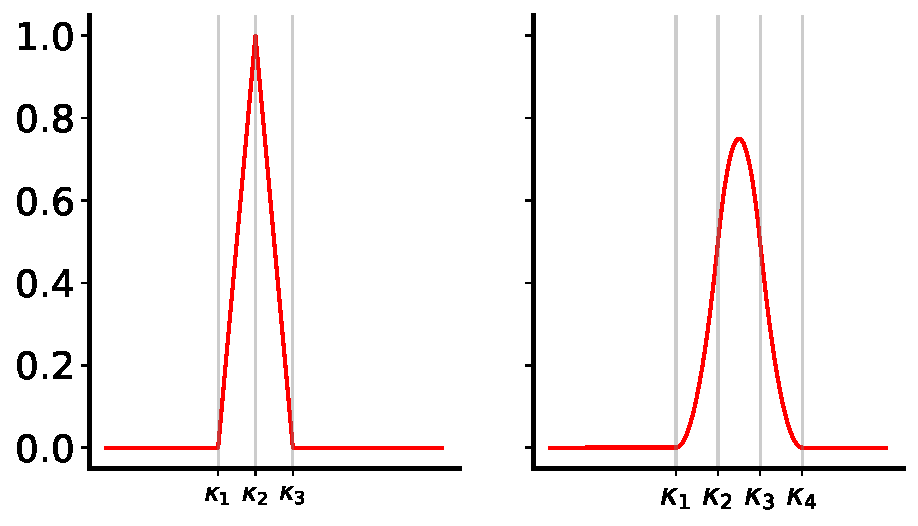
\includegraphics[width=\columnwidth]{../thesisplots/linear_and_quadratic_spline.pdf}
	\caption{Linear ($m=1$) and quadratic ($m=2$) spline}
	\label{fig:lin_and_quad_spline}
\end{figure}

The general properties of a B-spline of degree $m$ are the following:

\begin{itemize}
	\item It consists of $m+1$ polynomial pieces of degree $m$, e.g. a cubic spline ($m=3$) consists of 4 cubic pieces.
	\item The pieces join at $m$ inner knots.
	\item At these knots, the derivatives up to order $m-1$ are continuous.
	\item The B-spline is positive on the domain spanned by $m+2$ knots, everywhere else it is zero, e.g. for $m=2$, a sequence of 4 knots is necessary.
	\item At every given $x$, only $m+1$ B-splines are non-zero.
\end{itemize}

The collection of $k$ B-splines of degree $m$ over a sequence of $k+2(m-1)$ knots is called B-spline basis. The $2(m-1)$-knots are the boundary knots while the $k$ knots are the interior knots. The knots can either be an equidistant sequence, which facilitates the construction and estimation of the coefficients, or a non-equidistant sequence. \cite{eilers1996flexible}

A function $f(x)$ can then be represented using the basis function approach given by

\begin{align} \label{eq:bspline-bf-approach}
	f(x) = \sum_{i=1}^k B_i^m(x) \beta_i = \transpose{\vec{b}} \vec{\beta}
\end{align}

using the B-spline basis functions $B_i^m(x)$ of appropriate degree $m$ and the coefficient vector $\vec{\beta} \in \mathbb{R}^{k}$. The basis functions can be given in vector notation as $\transpose{\vec{b}} = (B_1^m(x), \dots, B_k^m(x))$. Using the set of data $\{ x^{(i)}, y^{(i)}\}, \ i=1, \dots, n$, the B-spline basis for $k$ splines of degree $m$ is given by the matrix $\vec{X}$ as

\begin{align} \label{eq:bspline-basis-matrix}
	\vec{X} = \begin{pmatrix}
				B_1^m(x^{(1)}) & \dots & B_k^m(x^{(1)})  \\
				\vdots         &       & \vdots 		 \\
				B_1^m(x^{(n)}) & \dots & B_k^m(x^{(n)})  \\
	\end{pmatrix} \ \mathbb{R}^{n \times k}
\end{align}

The linear combination of cubic B-splines gives a smooth function $f(x)$, i.e. first and second order derivatives are continuous. A further advantage of B-splines is that once the basis is given, the coefficients can be estimated using the Least Squares algorithm given in Chapter \ref{subsubsubsec:Method-of-LS}. 

Given a set of data points $\{x^{(i)}, y^{(i)}\}$ for $i = 1, \dots, n$, the least squares objective function for B-splines is the given by

\begin{align} \label{eq:OF_Bsplines}
	Q_{bsplines}(\vec{y}, \vec{\beta}) = \lVert \vec{y} - \vec{X} \vec{\beta} \rVert^2
\end{align}

for the B-spline basis matrix $\vec{X} \in \mathbb{R}^{n \times k}$ for $n$ data points and $k$ splines. Solving the optimization problem, i.e.

\begin{align} \label{eq:opti_problem_bsplines}
	\vec{\hat{\beta}} = \arg \min_{\vec{\beta}} Q_{bsplines}(\vec{y}, \vec{\beta})
\end{align}

leads to the estimated coefficients 

\begin{align}
	\vec{\hat{\beta}} = (\transpose{\vec{X}} \vec{X})^{-1} \transpose{\vec{X}} \vec{y}.
\end{align}

Therefore, the estimation is computationally efficient and easy to implement since closed-form solutions exists. Further, the advanced theoretical framework of linear models can be applied to use model selection and regularization approaches as well as to calculate e.g confidence intervals for the regression coefficients and the prediction.

B-splines of appropriate order $m > 2$ produce smooths curves, where the smoothness is mostly determined by the number of splines used. For a low number, the curve will be quite smooth, but possess a large data error. When using a high number of splines, the data error will be small but the variance of the curve will be large. This is an example of the bias-variance trade-off, a classical problem of regression and machine learning and further discussed in Chapter \ref{subsec:1d-function-estimation}. It is therefore necessary to introduce some kind of regularization. \cite{deBoor1978practicalGuideToSplines}  

%%%%%%%%%%%%%%%%%%%%%%%%%%%%%%%%%%%%%%%%%%%%%%%%%%%%%%%%%%%%%%%%%%%%%%%%%%%%%%%%%%%%%%%%%%%%%%%%%%%%%%%%%%%%%%%%%%
\subsection{P-Splines} \label{subsec:p-splines}

P-splines use the concepts of regularization to produce smooth function estimations. They where introduced by Eilers and Marx in \cite{eilers1996flexible} to tackle the problem stated above. Eilers and Marx simplified and generalized the idea of \cite{osullivan1986statistical}, who introduced a smoothness penalty based on the integral of the squared second derivative of the estimated spline to penalized wiggly function estimates. They proposed to use equidistant knot placement and a penalty based on finite differences of order $d$ of the coefficients of adjacent B-splines as approximation of the derivative.

The difference operator  $\Delta^d$ of order $d$ for equidistant knot placement of B-splines is defined by

\begin{align} \label{eq:difference-operators}
	\begin{split}
		\Delta^1 \beta_j &= \beta_j - \beta_{j-1} \\
		\Delta^2 \beta_j &= \Delta^1(\Delta^1 \beta_j) = \beta_j - 2\beta_{j-1} + \beta_{j-2} \\ 
		\vdots \\ 
		\Delta^d \beta_j &= \Delta^1(...(\Delta^1 \beta_j))
	\end{split}
\end{align}

and in matrix notation for order $d=1$

\begin{align} \label{eq:d1-difference-matrix}
	\vec{D}_1 = 
	\begin{pmatrix} 
		-1& 1&       &        &   \\  
		&-1& 1     &        &   \\  
		&  &\ddots & \ddots &   \\ 
		&  &       & -1     & 1 
	\end{pmatrix} \in \mathbb R^{k-1\times k}
\end{align}

and order $d=2$

\begin{align} \label{eq:d2-difference-matrix}
	\vec{D}_2 = 
	\begin{pmatrix} 
		1& -2& 1& &    \\  
		& 1 & -2 & 1& \\ 
		&  & \ddots & \ddots  & \ddots \\ 
		& & & 1 & -2 & 1 
	\end{pmatrix} \in \mathbb R^{k-2\times k}.
\end{align}

For non-equidistant knot placement, the difference operator $\Delta^1$ is defined according to \cite{ferziger2008numerische} as

\begin{align} \label{eq:d1-operator-nonequidistant}
	\Delta^1 \beta_j = \frac{\beta_j - \beta_{j-1}}{\delta_{j, j-1}}
\end{align}

with the denominator given by 

\begin{align} 
	\delta_{j, j-1} = \operatorname*{arg\, max}_x B_j^m(x) - \operatorname*{arg\, max}_x B_{j-1}^m(x).
\end{align}

The second order difference operator is further defined using the first order difference operator $\Delta^1$ as 

\begin{align} \label{eq:d2-operator-nonequidistant}
	\Delta^2 \beta_j = \frac{\Delta^1 \beta_{j+1} - \Delta^1 \beta_j}{\delta_{j+1,j}}.
\end{align}

In matrix form, the first order difference operator for non-equidistant knot placement is then given as

\begin{align} \label{eq:d1-matrix-nonequidistant}
	\vec{D_1} = \begin{pmatrix}
					\frac{-1}{\delta_{2,1}} & \frac{1}{\delta_{2,1}} &                         &  \\
										   & \frac{-1}{\delta_{3,2}} & \frac{1}{\delta_{3,2}} & \\
										   & 				        & 	\ddots                 & \ddots \\
										   &                        &                         & \frac{-1}{\delta_{k-1, k-2}} & \frac{1}{\delta_{k-1, k-2}} \\ 
	\end{pmatrix} \in \mathbb{R}^{k \times k-1}
\end{align} 

and the second order difference operator for non-equidistant knot placement is given as

\begin{align} \label{eq:d2-matrix-nonequidistant}
	\vec{D}_2 = \begin{pmatrix}
\frac{1}{\delta_{3,2} \delta_{2,1}} & \frac{- \delta_{3,1}}{\delta_{3,2}^2 \delta_{2,1}} & \frac{1}{\delta_{3,2}^2}  &  \\
									& \frac{1}{\delta_{4,3} \delta_{3,2}} & \frac{- \delta_{4,2}}{\delta_{4,3}^2 \delta_{3,2}} & \frac{1}{\delta_{4,3}^2} \\
									&       & 	\ddots    & \ddots & \ddots \\
		&    &  & \frac{1}{\delta_{k-1, k-2} \delta_{k-2, k-3}} & \frac{-\delta_{k-1, k-3}}{\delta_{k-1, k-2}^2 \delta_{k-2, k-3}} & \frac{1}{\delta_{k-1, k-2}^2} \\ 
	\end{pmatrix} \in \mathbb{R}^{k \times k-2}.
\end{align}


This leads to the penalized least squares formulation, similar to (\ref{eq:PLS_crit}),

\begin{align} \label{eq:OF_psplines}
	Q_{pslines}(\vec{y}, \vec{\beta}) = \lVert \vec{y} - \vec{X} \vec{\beta}\rVert^2 + \lambda_s \mathcal J_s(\vec{\beta};d)
\end{align}

where $\lVert \vec{y} - \vec{X} \vec{\beta} \rVert^2$ is the mean squared error on the data for the spline fit, $\mathcal J_s(\vec{\beta};d) = \transpose{\vec{\beta}} \transpose{\vec{D}}_d \vec{D}_d \vec{\beta}$ is the smoothness penalty term given by the matrix form of the difference operator $\Delta^d$ of order $d$ and $\lambda_s$ is the smoothness parameter determining the effect of the smoothness penalty. The estimated coefficients are then given by the minimization of

\begin{align}
	\vec{\hat{\beta}} = \arg \min_{\vec{\beta}} Q_{psplines}(\vec{y}, \vec{\beta})
\end{align}

using the penalized least squares algorithm as

\begin{align}
	\vec{\beta} = (\transpose{\vec{X}} \vec{X} + \lambda_s \transpose{\vec{D}}_d \vec{D}_d)^{-1} \transpose{\vec{X}} \vec{y}.
\end{align}

The main advantage of P-splines is their easy set up. This advantage is diminished if uneven knot placement is chosen, which is seen when comparing the matrix forms of the difference operators for the different knot placement types in e.g. (\ref{eq:d2-difference-matrix}) and (\ref{eq:d2-matrix-nonequidistant}). 

%%%%%%%%%%%%%%%%%%%%%%%%%%%%%%%%%%%%%%%%%%%%%%%%%%%%%%%%%%%%%%%%%%%%%%%%%%%%%%%%%%%%%%%%%%%%%%%%%%%%%%%%%%%%%%%%%%
\subsection{Tensor-Product Splines}

Tensor-product splines can be seen as the multi-dimensional extension of uni-variate B-splines. We start with a B-spline basis for each dimension and construct the tensor-product spline from these. 

We examine an example for two input dimensions $x_1$ and $x_2$. Assume that we have B-spline bases available, i.e. $\vec{A} \in \mathbb{R}^{n \times k}$ and $\vec{B} \in \mathbb{R}^{n \times k}$ using the same number of splines $k$ for both bases, for representing the functions $f_1(x_1)$ and $f_2(x_2)$ given by

\begin{align}
	f_1(x_1) &= \sum_{i=1}^{k} \alpha_i a_i(x_1) = \vec{A} \vec{\alpha}, \\
	f_2(x_2) &= \sum_{j=1}^{k} \beta_j b_j(x_2) = \vec{B} \vec{\beta}
\end{align}

where $\vec{\alpha} \in \mathbb{R}^{k}$ and $\vec{\beta} \in \mathbb{R}^{k}$ are the coefficients and $a_i(x_1)$ and $b_j(x_2)$ are the known basis functions. To allow the function $f_1(x_1)$ to smoothly vary with $x_2$, its coefficients $\alpha_i$ must vary smoothly with $x_2$. By using the already available basis for representing smooth functions in $x_2$, we can write

\begin{align}
	\alpha_i(x_2) = \sum_{j=1}^{k} \beta_{ij} b_j(x_2)
\end{align}

which leads to

\begin{align}
	f_{1,2}(x_1, x_2) = \sum_{i=1}^{k} \sum_{j=1}^{k} \beta_{ij} b_j(x_2) a_i(x_1).
\end{align}

We can therefore combine the individual basis matrices to generated a new basis matrix for the tensor-product spline. For any set of data $(x^{(i)}_{1}, x^{(i)}_{2})$ for $i = 1, \dots, n$, the relationship between the model matrix $\vec{X}$ of the tensor-product smooth and the marginal model matrices $\vec{A}$ and $\vec{B}$ is given by 

\begin{align}
	\vec{X} = \vec{A} \otimes \vec{B}
\end{align}

where $\otimes$ indicates the use of the Kronecker product, $\vec{X} \in \mathbb{R}^{n \times k^2}$ denotes the tensor-product spline basis, $\vec{A} \in \mathbb{R}^{n \times k}$ denotes the B-spline basis for dimension $x_1$ and $\vec{B} \in \mathbb{R}^{n \times k}$ denotes the B-spline basis for dimension $x_2$. The model matrix for the tensor-product smooth is therefore given by the Kronecker product of the marginal model matrices. \cite{wood2006GAM}  

This approach can in theory be continued for as much input dimensions as required. In practice, modeling more than two input dimensions using tensor-product splines becomes infeasible because of the enormous increase of basis functions and therefore coefficients to estimate. A smoothness penalty term for tensor-product splines can also be constructed using the Kronecker product. Further explanations are given in Chapter 3.

%%%%%%%%%%%%%%%%%%%%%%%%%%%%%%%%%%%%%%%%%%%%%%%%%%%%%%%%%%%%%%%%%%%%%%%%%%%%%%%%%%%%%%%%%%%%%%%%%%%%%%%%%%%%%%%%%%
%%%%%%%%%%%%%%%%%%%%%%%%%%%%%%%%%%%%%%%%%%%%%%%%%%%%%%%%%%%%%%%%%%%%%%%%%%%%%%%%%%%%%%%%%%%%%%%%%%%%%%%%%%%%%%%%%%
\section{Structured Additive Regression} \label{sec:STAR}

We have again some given data $\{x^{(i)}_{1}, \dots, x^{(i)}_{q}; y^i\}$ for $i = 1, \dots, n$ and want to model the generally non-linear relationship between the input data $\{x^{(i)}_{1}, \dots, x^{(i)}_{q}\}$ and the output $y^{(i)}$ by some multi-dimensional function $f(x_1, \dots, x_q)$.  Using, e.g. high-dimensional tensor-product splines, to model the function is computationally expensive, since the number of regression coefficients increases exponentially.

To circumvent this problem, we now assume the restrictive structure of additive models, given by

\begin{align} \label{eq:addRegBaseEquation}
	f(x_1, \dots, x_q) = f_1(x_1) + \dots + f_q(x_q).
\end{align}

Hence, we use one smooth function $f_i(x_i)$ per input dimension and assume an additive structure. \cite{fahrmeir2013regression} Using the concepts introduced in Chapter \ref{sec:Splines}, we obtain for each smooth function a linear model

\begin{align}
	f_i(\vec{x}_i) = \vec{X}_i \vec{beta}_i
\end{align}

where $\vec{X}_i \in \mathbb R^{n \times k_i}$ is the B-spline basis using $k_i$ splines for the smooth function $f_i(x_i)$ of input dimension $i$, $\vec{x}_i = (x_i^{(1)}, \dots, x_i^{(n)})$ is the data vector of input dimension $i$ and $\vec{\beta}_i \in \mathbb R^{k_i}$ are the coefficients to be estimated. We can also use the already described penalization approaches given in Chapter \ref{subsec:p-splines}. 

The model given in (\ref{eq:addRegBaseEquation}) does not contain interaction terms between variables. Nevertheless, these can be easily introduced for 2 dimensions using tensor-product splines without an overflowing increase in the number of coefficients.

We can then write the structured additive model in matrix notation as 

\begin{align} \label{eq:STAR}
	\vec{y} = \vec{X}_1 \vec{\beta}_1 + \dots + \vec{X}_q \vec{\beta}_q + \sum_{i=1}^{n_{interact}} \vec{X}_{tps, i} \vec{\beta}_{tps,i} + \vec{\epsilon}
\end{align}

using the error term $\vec{\epsilon} \in \mathbb{R}^n$ and $n_{interact}$ as the number of interactions to include via tensor-product spline bases $\vec{X}_{tps,i} \in \mathbb{R}^{n \times k_i^2}$. This can be solved using ordinary least squares. If we choose to include penalization, we can solve this using penalized least squares. 

Using the notation in (\ref{eq:STAR}) the theoretical framework of linear models can be applied to structured additive regression models. Therefore, the assumptions given in Chapter \ref{subsec:LinModelDefAndAssump} on the error term, as well as on the model functions are used. \cite{fahrmeir2004penalized}

\chapter{Solution Approach}

We are now going to use the theory discussed in Chapter 2 to estimate functions using available data and a priori domain knowledge. An overview of the different problems considered in this work is given in Table \ref{tab:problem_overview}. First, we are using B-splines, see Chapter \ref{subsec:b-splines}, as basis functions for the estimation of the unknown function $y = f(x)$ for some data $\{x^{(i)}, y^{(i)}\} \ i = 1, \dots, n$.  Next, we use the concept of P-splines, see \ref{subsec:p-splines},  introduced by Eilers and Marx in \cite{eilers1996flexible} to estimate smooth, one dimensional functions. Finally, we are going to incorporate a priori knowledge into the fitting process using the approach given by Hofner and apply it to one and two dimensional functions. \cite{hofner2011monotonicity} 

\begin{table}[H]
	\centering
	\begin{tabular}{|lll|}
		\hline
		\textbf{Problem}                   & \textbf{Solution Approach}           & \textbf{Algorithm}  \\ \hline \toprule
		1d Function Estimation             & B-Splines                            & LS                  \\ \hline
		1d Smooth Function Estimation      & P-Splines                            & PLS                 \\ \hline
		1d Constraint Function Estimation  & P-Splines + Constraint Penalty       & PIRLS 			    \\ \hline 
		n-d Constraint Function Estimation & P+TP-Splines + Constraint Penalty & PIRLS 			    \\ \hline \bottomrule
	\end{tabular}
	\caption{Problem overview}
	\label{tab:problem_overview}
\end{table}

The a priori knowledge can be incorporated using different types of constraints. The considered constraints are listed in Table \ref{tab:constraint_overview}.

\begin{table}[h]
	\centering
	\begin{tabular}{|lll|}
		\hline
		\textbf{Constraint}& \textbf{Description}                         & \textbf{Math. Description}\\ \hline \toprule
		Monotonicity       & Functions is either increasing or decreasing.& $\lvert f'(x) \rvert \ge 0$ 	\\ \hline
		Curvature          & Function is either convex or concave.        & $\lvert f''(x) \rvert \ge 0$ 	\\ \hline
		Unimodality        & Function has a mode/peak.                    & $m = \arg \max_{x} f(x)$ 				\\ 
		&	   										  & $f'(x) \ge 0 \quad \text{if} \ x < m$  \\ 
		&  											  & $f'(x) \le 0 \quad \text{if} \ x > m$  \\ \hline
		Boundedness        & Function is bounded by the value M.          & $\lvert f(x)\rvert \le M$ 		\\ \hline
		Jamming            & Function is jammed by the value M.           & $f(x^{(M)}) \approx y^{(M)}$	\\ \hline \bottomrule
	\end{tabular}
	\caption{Overview of the considered constraints}
	\label{tab:constraint_overview}
\end{table}

To test the algorithm and the incorporation of a priori knowledge, we use the one dimensional function given by 

\begin{align}\label{eq:test_func}
	f(x) = 3\sin(3\pi x) + 17x + 3.
\end{align}

Figure \ref{fig:test_func} shows functions evaluated at 200 points. The function is partially increasing.  

\begin{figure}[H]
	\centering
	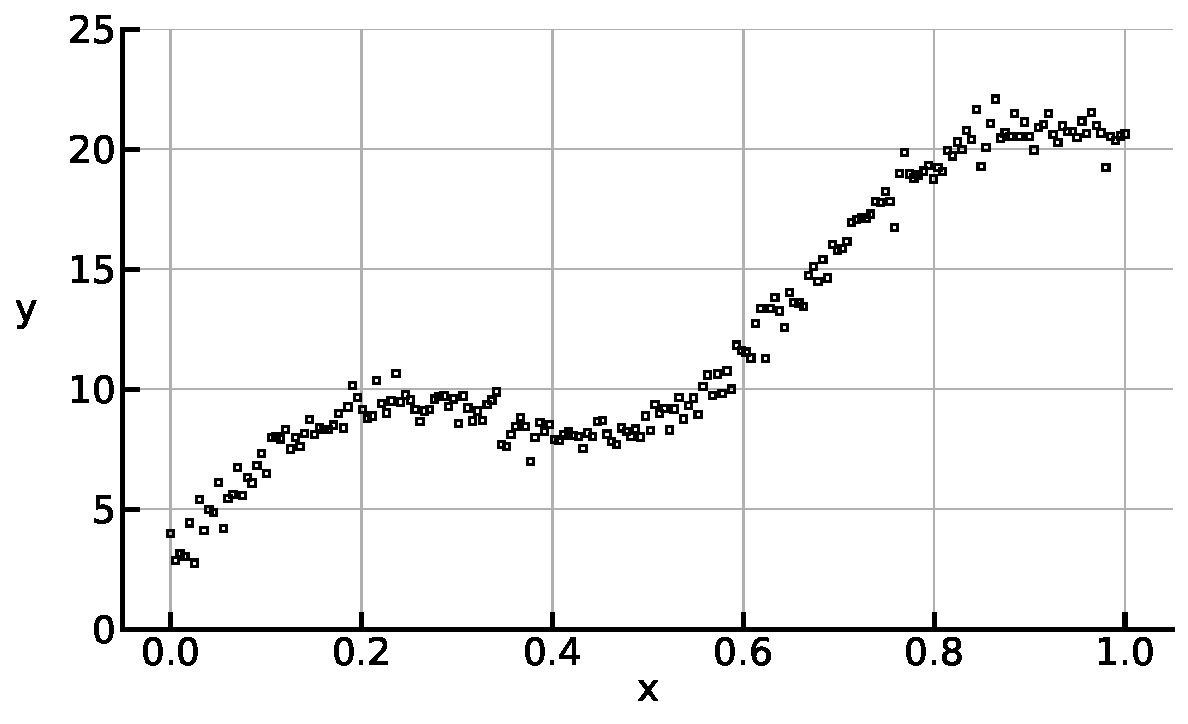
\includegraphics[width=\columnwidth]{../thesisplots/test_func.pdf}
	\caption{Noisy samples determined from test function (\ref{fig:test_func})}
	\label{fig:test_func}
\end{figure}

%%%%%%%%%%%%%%%%%%%%%%%%%%%%%%%%%%%%%%%%%%%%%%%%%%%%%%%%%%%%%%%%%%%%%%%%%%%%%%%%%%%%%%%%%%%%%%%%%%%%%%%%%%%%%%%%%
\section{Function Estimation}

\subsection{1d Function Estimation} \label{subsec:1d-function-estimation}

The goal is to model given data

\begin{align} \label{eq:data}
	\{\vec{x}, \vec{y}\} = \{x^{(i)}, y^{(i)}\}, \ i = 1, \dots, n 
\end{align}

using B-splines as basis functions. Therefore we want to estimate the unknown function $\vec{y} = f(\vec{x})$, which can be represented as a linear combination of $k$ B-spline basis functions $B_j^m$ of degree $m=3$, cf. (\ref{eq:bspline-bf-approach}), as

\begin{align} \label{eq:basis_function_approach}
	\vec{y} = \vec{X} \vec{\beta},
\end{align}

where $\vec{X} \in \mathbb{R}^{n\times k}$ is the B-spline basis matrix, cf. (\ref{eq:bspline-basis-matrix}), and $\vec{\beta} \in \mathbb{R}^k$ are the coefficients to be estimated. 

The least squares objective function to be minimized using the complete data is then given by

\begin{align} \label{eq:OF_1}
	Q_1(\vec{y}, \vec{\beta}) = \lVert \vec{y} - f(\vec{x}) \rVert^2 = \lVert \vec{y} - \vec{X}\vec{\beta} \rVert^2 
\end{align}	

The coefficients are determined by minimizing the objective function $Q_1$ given in (\ref{eq:OF_1}) with respect to $\vec{\beta}$, i.e.

\begin{align}\label{eq:optimization_problem_1}
	\vec{\hat \beta}_{LS} = \arg \min_{\vec{\beta}} Q_1(\vec{y}, \vec{\beta}).
\end{align}

Using the least squares algorithm LS, see Chapter \ref{subsubsubsec:Method-of-LS}, the minimization problem (\ref{eq:optimization_problem_1}) yields 

\begin{align} \label{eq:LS_coef}
	\vec{\hat \beta}_{LS}= (\transpose{\vec{X}} \vec{X})^{-1} \transpose{\vec{X}} \vec{y}.
\end{align} 


Figure \ref{fig:smooth_bf} shows a B-spline model using $k=10$ splines on an equidistant grid approximating the noisy data presented in Figure \ref{fig:test_func}, as well as the individual B-spline basis functions $B_i^3(\vec{x})$ multiplied with the corresponding, estimated coefficients $\vec{\hat \beta}_{LS, j} \ j=1, \dots, 10$.

\begin{figure}[H]
	\centering
	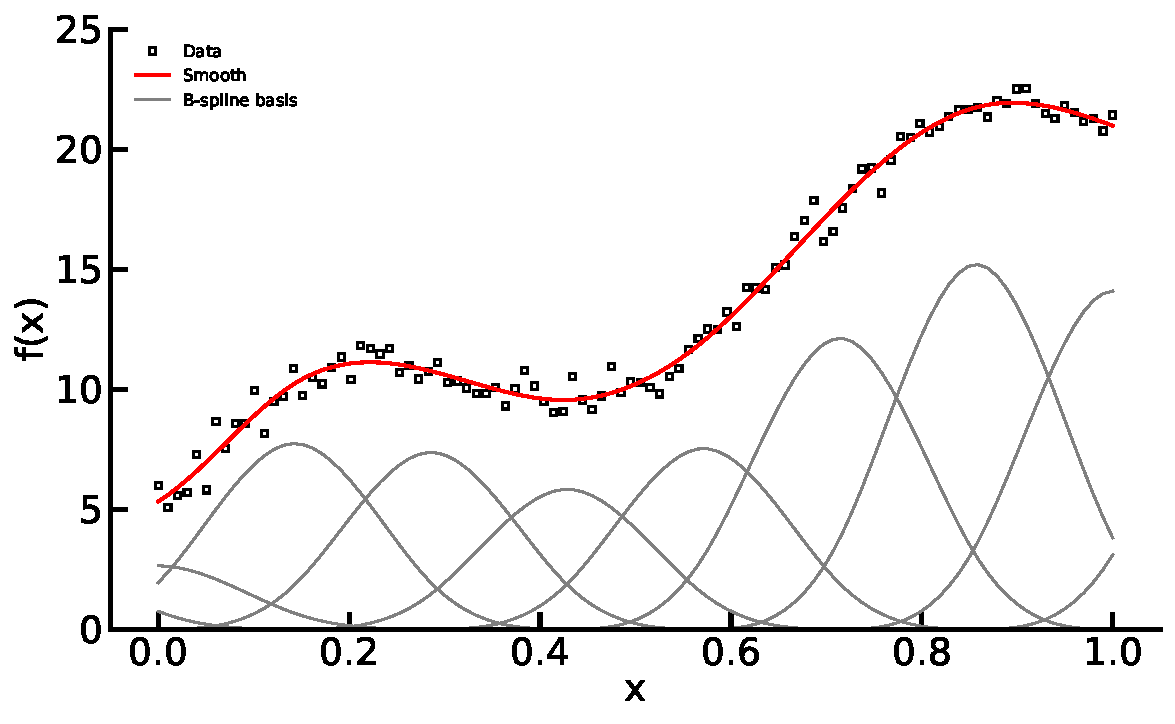
\includegraphics[width=\columnwidth]{../thesisplots/smooth_bf.pdf}
	\caption{Approximation of the noisy data by B-splines without constraints}
	\label{fig:smooth_bf}
\end{figure}


Note, the number of splines $k$ has a strong influence on the amount of smoothing. A small number $k$ leads to a very smooth estimate, but a large data error. On the other hand, when the number of splines is relatively large, the data error is very small but the smoothness of the estimate is poor. This behavior is an example of the well-known bias-variance dilemma and depicted in Figure \ref{fig:smooth_bf_large}. \cite{sammut2011}
Here, two B-splines models with $k=10$ and $k=50$ are illustrated, which are applied to the noisy data shown in Figure \ref{fig:test_func}. To overcome this challenges, the B-splines will be extended by penalizing the second derivative of the estimation, see Chapter \ref{subsec:1D_smooth}. 

\begin{figure}[H]
	\centering
	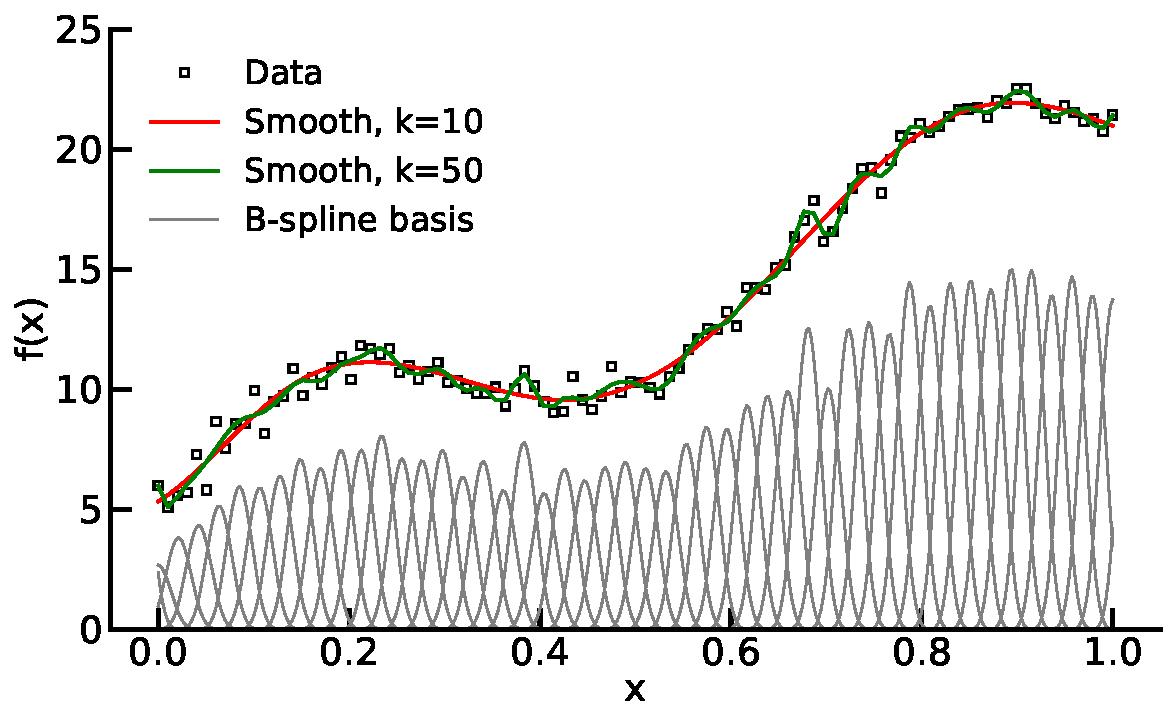
\includegraphics[width=\linewidth]{../thesisplots/smooth_wiggly_bf.pdf}
	\caption{Approximation of the noisy data by 10 and 50 B-splines without constraints}
	\label{fig:smooth_bf_large}
\end{figure}


%%%%%%%%%%%%%%%%%%%%%%%%%%%%%%%%%%%%%%%%%%%%%%%%%%%%%%%%%%%%%%%%%%%%%%%%%%%%%%%%%%%%%%%%%%%%%%%%%%%%%%%%%%%%%%%%%
\subsection{1d Smooth Function Estimation} \label{subsec:1D_smooth}

The second derivative of the estimated function $f(x)$, i.e. $f''(x) = \sum_{j=1}^k B''_i(x) \beta_k$, has to be penalized to realize a smoother estimate when using  a high number of splines. Eilers and Marx have introduced the so-called P-splines. \cite{eilers1996flexible}, see Chapter \ref{subsec:p-splines}. Therefore, the objective function (\ref{eq:OF_1}) is extended by an additional term considering the smoothness, i.e.

\begin{align}\label{eq:OF_2}
	Q_2(\vec{y}, \vec{\beta}) = Q_1(\vec{y}, \vec{\beta}) + \lambda_s \mathcal{J}_s(\vec{\beta}; d) = \lVert \vec{y} - \vec{X} \vec{\beta} \rVert^2 + \lambda_s \transpose{\vec{\beta}} \transpose{\vec{D}}_d \vec{D}_d \vec{\beta}, 
\end{align}

with the smoothing parameter $\lambda_s$ and an appropriate mapping matrix $\vec{D}_d$ capturing the second derivative, which itself is a measure for function wiggliness. Here, an approximation of the second derivative can be performed by the squared finite difference of order $d$ of adjacent coefficients using the matrix form of the difference operator of order $d$, see Chapter \ref{subsec:p-splines}. 

By minimizing the objective function (\ref{eq:OF_2}), i.e.

\begin{align}\label{eq:optimization_problem_2}
	\vec{\hat \beta}_{PLS} = \arg \min_{\vec{\beta}} Q_2(\vec{y}, \vec{\beta}),
\end{align}

using the penalized least squares algorithm PLS, the penalized least squares coefficients are given by

\begin{align} \label{eq:PLS_coef}
	\vec{\hat \beta}_{PLS}= (\transpose{\vec{X}} \vec{X} + \lambda_s \transpose{\vec{D}}_d \vec{D}_d)^{-1} \transpose{\vec{X}} \vec{y}.
\end{align} 

In (\ref{eq:PLS_coef}), the smoothing parameter $\lambda_s$ plays a critical role and can be optimized using the information criteria specified in Chapter Model Selection Criteria, e.g. AIC and BIC, or by using cross-validation techniques. \cite{fahrmeir2013regression}
For small values $\lambda_s \rightarrow 0$, the penalized least squares estimate $\vec{\hat{\beta}}_{PLS}$ approaches the least squares estimate $\vec{\hat{\beta}}_{LS}$, cf. (\ref{eq:LS_coef}), while for large values $\lambda_s \gg 0$, the fitted function shows the behavior of a polynomial with $d-1$ degrees of freedom. For example, using $d=2$ and a large smoothing parameter $\lambda_s$ this configuration leads to a linear function, while using $d=1$ would lead to a constant function. \cite{fahrmeir2013regression}

Figure \ref{fig:psplines} shows the behavior of P-splines using $k=50$ splines for several values of the smoothing parameter $\lambda_s = \{10^{-2}, 10^{2},10^{5},10^{6}\}$ and a smoothness penalty of order $d=2$.  As the value of $\lambda_s$ gets larger, the fitted curve becomes more smooth and thus the $2^{nd}$ derivative of the curve becomes smaller due to the penalty considered in the estimation, see (\ref{eq:PLS_coef}). For very large values of $\lambda_s$, the estimate approaches a straight line, see the yellow curve in Figure \ref{fig:psplines}.

\begin{figure}[H]
	\centering
	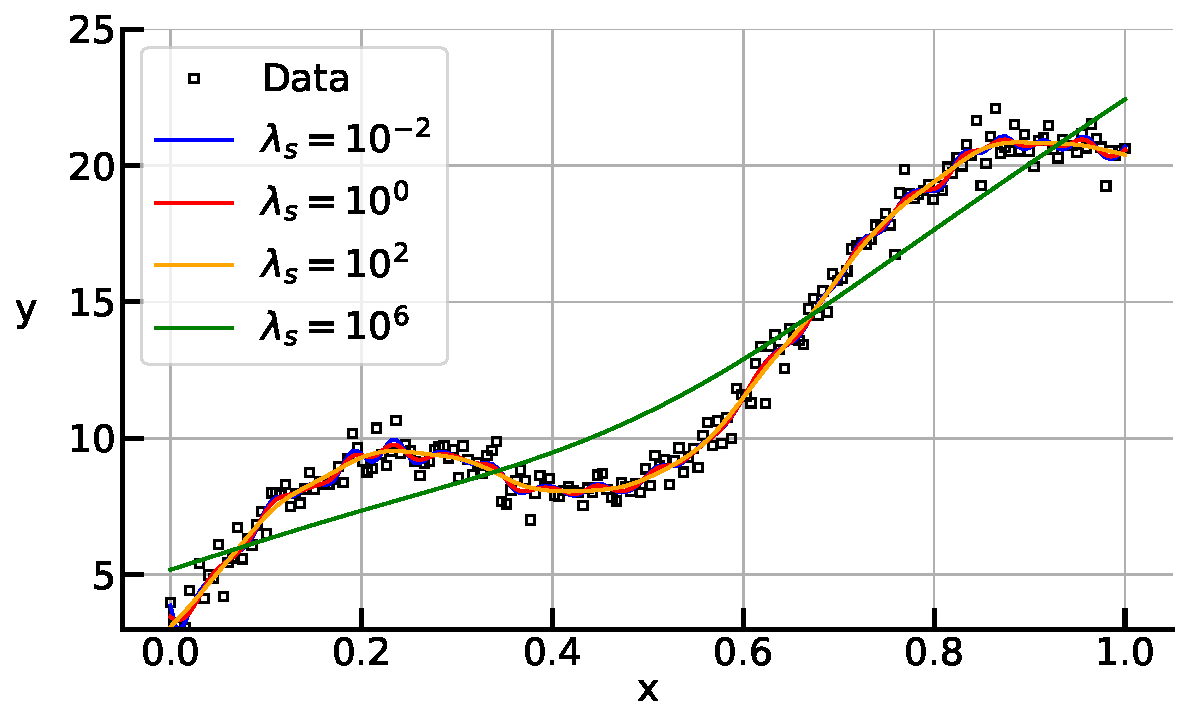
\includegraphics[width=\linewidth]{../thesisplots/p_splines.pdf}
	\caption{Smooth function estimation for different smoothing parameters $\lambda_s$}
	\label{fig:psplines}
\end{figure}

%%%%%%%%%%%%%%%%%%%%%%%%%%%%%%%%%%%%%%%%%%%%%%%%%%%%%%%%%%%%%%%%%%%%%%%%%%%%%%%%%%%%%%%%%%%%%%%%%%%%%%%%%%%%%%%%%
\subsection{1d Constraint Function Estimation}

A priori domain knowledge can now be systematically considered by the extension of the objective function (\ref{eq:OF_2}) using an additional term representing the user-defined constraint, see Table \ref{tab:constraint_overview}. Note that this approach incorporates the a priori knowledge as soft constraints. Therefore, no guarantee can be given that the fit holds the constraint for every possible input. The constraint penalized least-squares objective function is given by

\begin{align}\label{eq:OF_3}
	Q_3(\vec{y}, \vec{\beta}) = Q_1(\vec{y}, \vec{\beta}) + \lambda_s \mathcal{J}_s(\vec{\beta}; d) + \lambda_c \mathcal{J}_c(\vec{\beta}; c)
\end{align}

with the corresponding constraint parameter $\lambda_c$, which determines the influence of the user-defined constraint. Note that the parameter $\lambda_c$ has to be set quite large, i.e. $\lambda_c > 10^4$, compared to $\lambda_s$ to enforce the user-defined constraint. 

Constraints for monotonicity, curvature, unimodality, boundedness and jamming can be modeled as 

\begin{align} \label{eq:mapping_matrix}
	\mathcal{J}_c(\vec{\beta}; c) = \transpose{\vec{\beta}} \transpose{\vec{D}}_c \vec{V} \vec{D}_c  \vec{\beta}
\end{align}

with the mapping matrix $\vec{D}_c$ and the diagonal weighting matrix $\vec{V} := \vec{V}(\vec{\beta}; c)$ capturing if the constraint $c$ is active or inactive. The matrices $\vec{D}_c$ and $\vec{V}$ will further be defined in Chapter \ref{sec:user-defined-constraints}.

By minimizing the objective function (\ref{eq:OF_3}), i.e.

\begin{align}\label{eq:optimization_problem_3}
	\vec{\hat \beta}_{PLS, c} = \arg \min_{\vec{\beta}} Q_3(\vec{y}, \vec{\beta}),
\end{align}

the constraint penalized least-squares estimate can be given as

\begin{align} \label{eq:PLS,c_coef}
	\vec{\hat \beta}_{PLS, c} = (\transpose{\vec{X}} \vec{X} + \lambda_s \transpose{\vec{D}}_d \vec{D}_d + \lambda_c \transpose{\vec{D}}_c \vec{V} \vec{D}_c)^{-1} \transpose{\vec{X}} \vec{y}.
\end{align}	

Note, (\ref{eq:PLS,c_coef}) is a nonlinear equation because the matrix $\vec{V}$ depends on $\vec{\beta}$. Thus, it has to be solved iteratively to calculate optimal coefficients $\hat{\vec{\beta}}_{PLS,c}$. The algorithm is shown in Figure \ref{fig:pirls}. 

\begin{figure}[H]
	\centering
	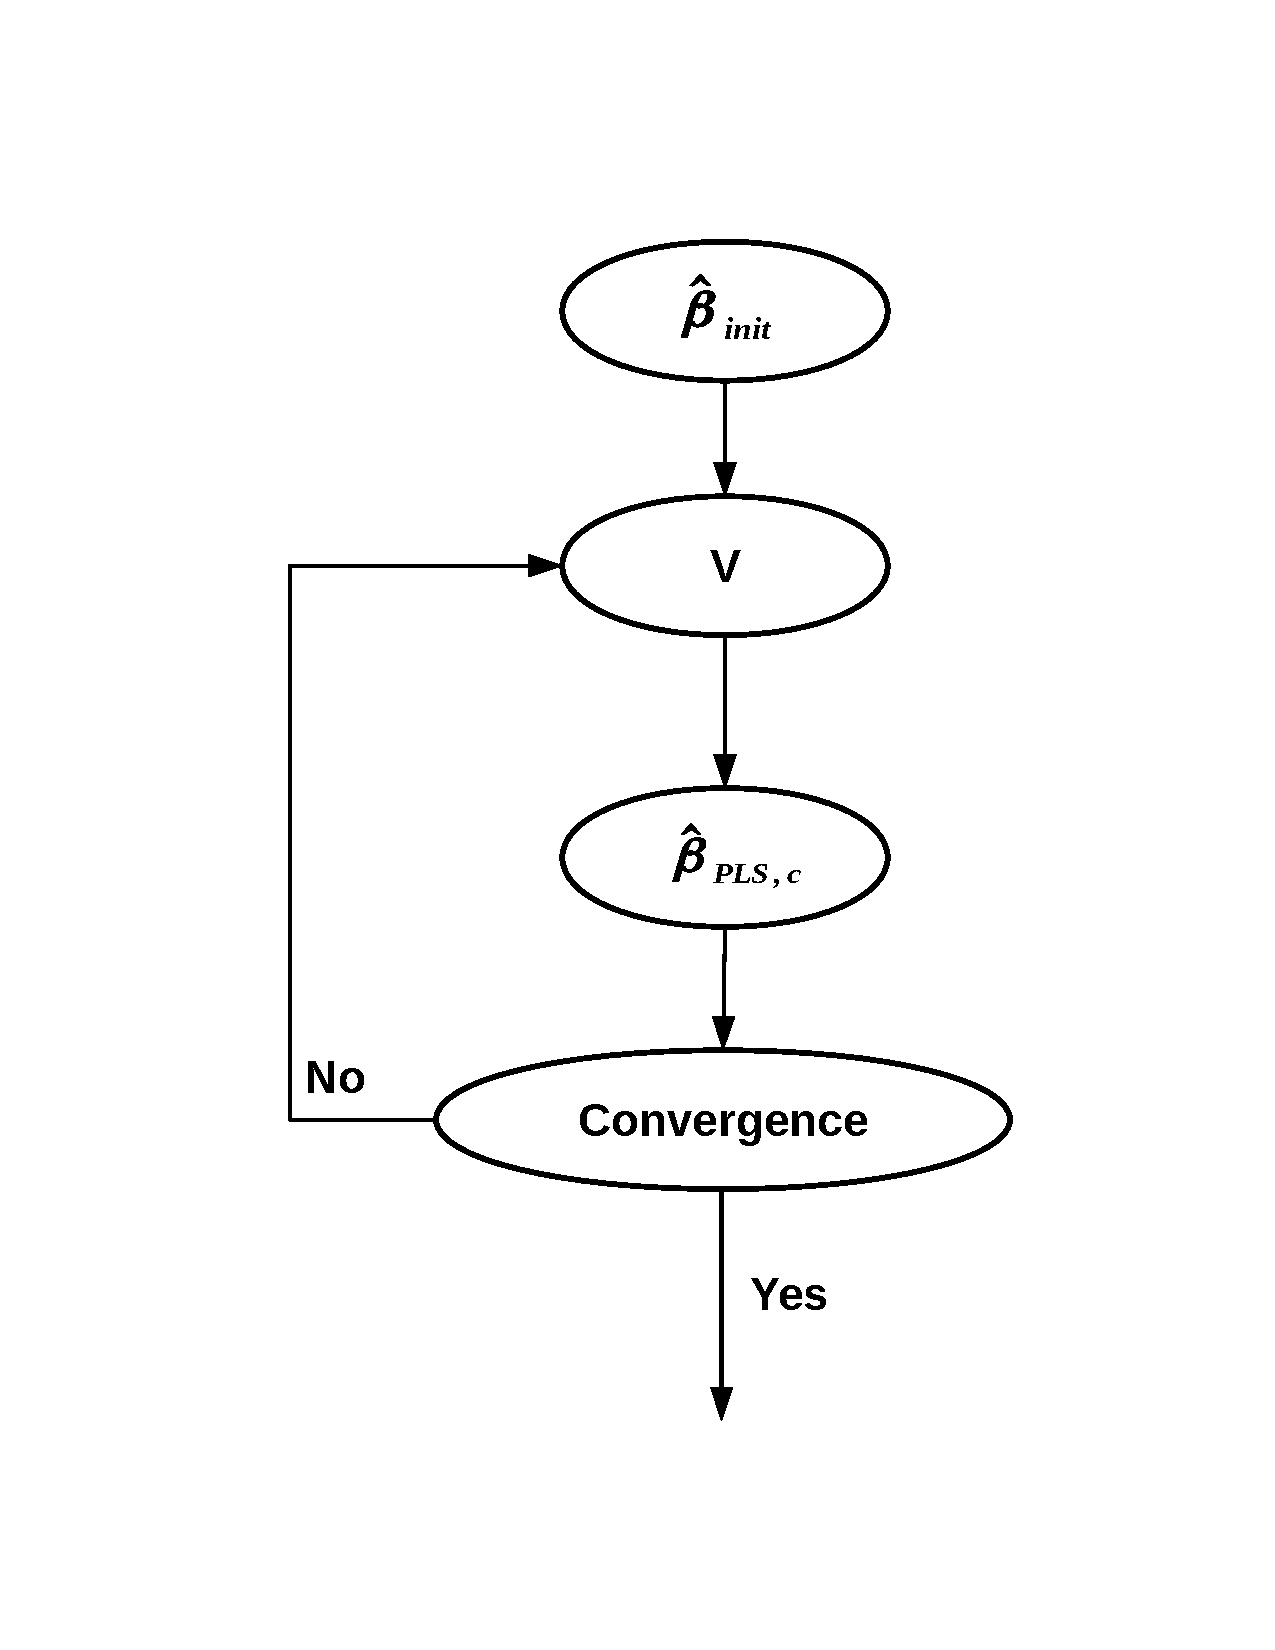
\includegraphics[width=0.6\linewidth]{../thesisplots/algorithm.pdf}
	\caption{Penalized iteratively reweighted least squares algorithm}
	\label{fig:pirls}
\end{figure}


The initial estimate $\vec{\hat{\beta}}_{init}$ needed to compute the weighting matrix $\vec{V}$ is given by the least squares estimate $\hat{\vec{\beta}}_{LS}$. Based on the initial estimate $\hat{\vec{\beta}}_{init}$, the weighting matrix $\vec{V}$ and then the constraint least-squares estimate $\hat{\vec{\beta}}_{PLS,c}$ are calculated. The algorithm is performed until no more changes in the weighting matrix $\vec{V}$ appear. This scheme is called the penalized iteratively reweighted least squares and is abbreviated by PIRLS. \cite{hofner2011monotonicity}


Figure \ref{fig:incspline} shows an example, where the noisy data shown in Figure \ref{fig:test_func} is approximated by considering the monotonicity constraint. The estimate has to be monotonically increasing in contrast to the data, i.e. $f'(x) \ge 0$.  The smoothing parameter $\lambda_s$ was optimized using cross-validation and set to $\lambda_s=271.9$. The constraint parameter $\lambda_c$ was set to $\lambda_c = 6000$. For both function estimations, the number of used splines $k$ was set to $k=30$. 	

\begin{figure}[H]
	\centering
	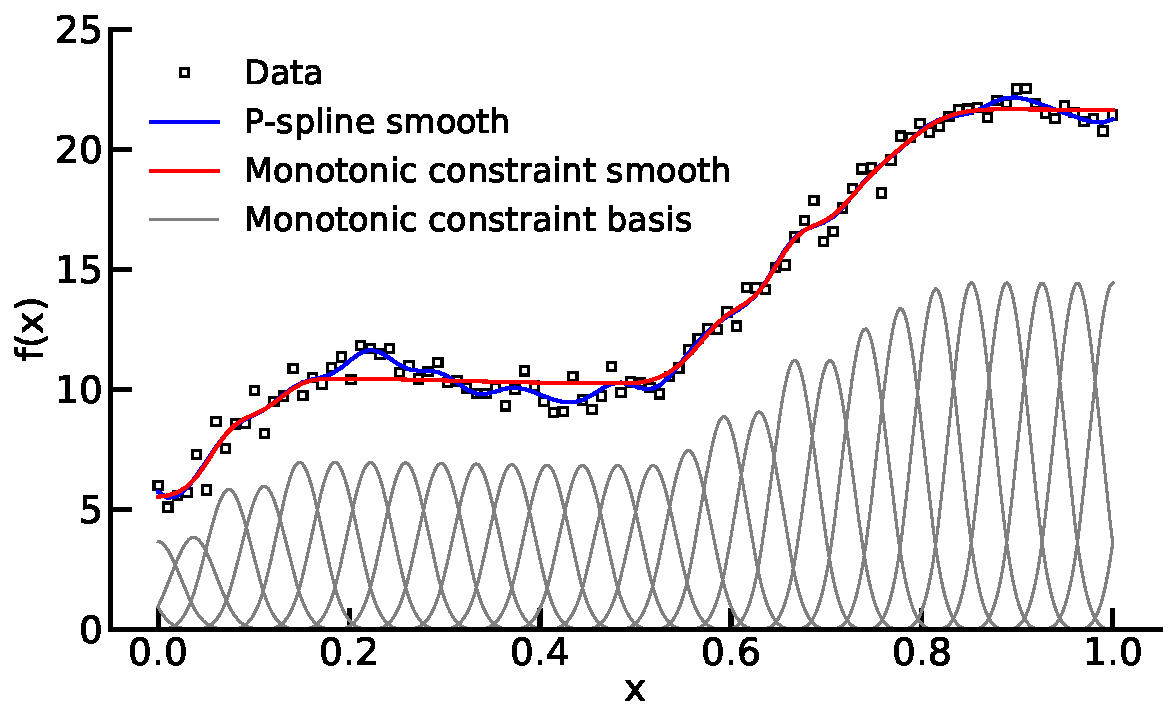
\includegraphics[width=\linewidth]{../thesisplots/inc_spline.pdf}
	\caption{Approximation of the noiy data by P-splines and P-splines with the monotonic increasing constraint}
	\label{fig:incspline}
\end{figure}	

The constraint function estimation (red curve in Figure \ref{fig:incspline}), follows the monotonicity constraint far better that the smooth function estimation (blue curve in Figure \ref{fig:incspline}). For $x < 0.15$ and $x > 0.6$, the two fits are nearly identical, since no constraint violation is present. Note, the entries of the weighting matrix $\vec{V}$ in this region are therefore $0$ everywhere because the constraint is not active. For $x \in [0.15, 0.6]$ the constraint is active. The red fit produces an almost constant line in this region as an optimal solution for the competing goals of data accuracy, smoothness and constraint fidelity.

This shows, that the incorporation of a priori knowledge in the fitting process using P-splines is in principle possible using an appropriate choice of the mapping matrix $\vec{D}_c$ and the weighting matrix $\vec{V}$ as well as an iterative fitting approach using penalized iteratively reweighted least squares. 

%%%%%%%%%%%%%%%%%%%%%%%%%%%%%%%%%%%%%%%%%%%%%%%%%%%%%%%%%%%%%%%%%%%%%%%%%%%%%%%%%%%%%%%%%%%%%%%%%%%%%%%%%%%%%%%%%
%%%%%%%%%%%%%%%%%%%%%%%%%%%%%%%%%%%%%%%%%%%%%%%%%%%%%%%%%%%%%%%%%%%%%%%%%%%%%%%%%%%%%%%%%%%%%%%%%%%%%%%%%%%%%%%%%	
\section{User-defined Constraints} \label{sec:user-defined-constraints}

As stated before, a priori domain knowledge given in Table \ref{tab:constraint_overview} can be introduced by the choice of the mapping matrix $\vec{D}_c$ and the weighting matrix $\vec{V}$, cf. (\ref{eq:mapping_matrix}) and (\ref{eq:PLS,c_coef}). Now a description of the different matrices, which are used to enforce a priori known behavior, is presented. 

%%%%%%%%%%%%%%%%%%%%%%%%%%%%%%%%%%%%%%%%%%%%%%%%%%%%%%%%%%%%%%%%%%%%%%%%%%%%%%%%%%%%%%%%%%%%%%%%%%%%%%%%%%%%%%%%%
\subsection{Monotonicity Constraint}

The mapping matrix $\vec{D}_c^{monoton}$ enforcing monotonic behavior follows from the first order difference operator $\Delta^1$ for equidistant knot placement, cf. \ref{eq:d1-difference-matrix}. The corresponding matrix for $k$ splines is given as

\begin{align} \label{eq:D_c_monoton}
	\vec{D}_c^{monoton} = \begin{pmatrix}  -1 & 1  &  		& \\ 
		& -1 & 1 		& \\ 
		&    & \ddots  & \ddots  
	\end{pmatrix} \in \mathbb{R}^{k-1 \times k}.
\end{align}

The difference between monotonic increasing and decreasing behavior is controlled by the weighting matrix $\vec{V}$. For increasing behavior, the weighting matrix $\vec{V}$ is given by the weights $v_j$ according to

\begin{align} \label{eq:v_monoton_inc}
	v_j(\vec{\beta}) = \begin{cases}
			0, \quad \text{if} \ \Delta^1\beta_j \ge 0 \\ 
			1, \quad \text{if} \ \Delta^1\beta_j < 0
	\end{cases}	
\end{align}

for $j=2, \dots, k$. 

For decreasing behavior, the weighting matrix $\vec{V}$ is given by the weights $v_j$ according to
\begin{align} \label{eq:v_monoton_dec}
	v_j(\vec{\beta}) = \begin{cases} 0, \quad \text{if} \ \Delta^1\beta_j \le 0 \\ 
		1, \quad \text{if} \ \Delta^1\beta_j > 0
	\end{cases}	
\end{align}

for $j=2, \dots, k$.

This states, that the penalty term $\mathcal{J}_c(\vec{\beta}; c)$ only contributes if adjacent coefficients $\beta_{j-1}$ and $\beta_j$ are increasing or decreasing, respectively. \cite{hofner2011monotonicity} \cite{eilers2005unimodal}

%%%%%%%%%%%%%%%%%%%%%%%%%%%%%%%%%%%%%%%%%%%%%%%%%%%%%%%%%%%%%%%%%%%%%%%%%%%%%%%%%%%%%%%%%%%%%%%%%%%%%%%%%%%%%%%%%	
\subsection{Curvature Constraint}

In the simplest case, the curvature of the function $f(x)$ can either be convex, i.e. $f''(x) \ge 0$, or concave, i.e. $f''(x) \le 0$. The mapping matrix $\vec{D}_c^{curvature}$ enforcing this behavior can be approximated by the second order difference operator $\Delta^2$ for equidistant knot placement, cf. (\ref{eq:d2-difference-matrix}). The corresponding matrix for $k$ splines is given as

\begin{align} \label{eq:D_c_curvature}
	\vec{D}_c^{curvature} = \begin{pmatrix} 1 & -2 & 1 		&  		 & \\ 
		& 1  &-2 	    &1 		 & \\
		& 	  & \ddots  & \ddots & \ddots  
	\end{pmatrix} \in \mathbb{R}^{k-2 \times k}.
\end{align}	

The difference between concave and convex curvature is controlled by the weighting matrix $\vec{V}$. For concave curvature, the weighting matrix $\vec{V}$ is given by the weights $v_j$ according to

\begin{align}\label{eq:v_curvature_concave}
	v_j(\vec{\beta}) = \begin{cases} 
		0, \quad \text{if} \ \Delta^2\beta_j \le 0 \\ 
		1, \quad \text{if} \ \Delta^2\beta_j > 0. 
	\end{cases}
\end{align}

For convex curvature, the weighting matrix $\vec{V}$ is given by the weights $v_j$ according to

\begin{align}\label{eq:v_curvature_convex}
	v_j(\vec{\beta}) = \begin{cases} 
		0, \quad \text{if} \ \Delta^2\beta_j \ge 0 \\ 
		1, \quad \text{if} \ \Delta^2\beta_j < 0. 
	\end{cases}
\end{align}	

Therefore, the penalty term $\mathcal{J}_c(\vec{\beta}; c)$ in (\ref{eq:OF_3}) or (\ref{eq:PLS,c_coef}) only contributes if the second order difference of adjacent coefficients $\vec{\beta}$ is either positive or negative, respectively. \cite{eilers2005unimodal}

%%%%%%%%%%%%%%%%%%%%%%%%%%%%%%%%%%%%%%%%%%%%%%%%%%%%%%%%%%%%%%%%%%%%%%%%%%%%%%%%%%%%%%%%%%%%%%%%%%%%%%%%%%%%%%%%%	
\subsection{Unimodality Constraint}

A function $f(x)$ is said to be unimodal if for some value $m$, it is monotonically increasing for $x \le m$ and monotonically decreasing for $x \ge m$. We assume that there is a peak in the data $\{x^{(i)}, y^{(i)}\}$ and therefore want to constrain the fit to include a peak.

The mapping matrix $\vec{D}_c^{unimodal}$ enforcing unimodal behavior can be constructed using the first order difference operator $\Delta^1$ for equidistant knot placement, cf. (\ref{eq:d1-difference-matrix}). The weighting matrix $\vec{V}$ now has a special structure. 

First, we construct the B-spline basis according to the given data as in Chapter \ref{subsec:b-splines}. We then need to find the index $j_{peak}$ of the \emph{peak spline}, which has the maximal value at the peak data point $\max \{f(x^{(j)}) \forall j\}$, see Figure \ref{fig:peak_spline}. The index $j_{peak}$ is now used as splitting point for the weighting matrix $\vec{V}$. All coefficients $\beta_j$ for $j < j_{peak}$ are constrained to be monotonic increasing, i.e. $\Delta^1 \beta_j \ge 0$ for $j = 1, \dots, j_{peak}-1$, while all coefficients $\beta_j$ for $j > j_{peak}$ are constrained to be monotonic decreasing, i.e. $\Delta^1 \beta_j \le 0$ for $j = j_{peak}+1, \dots, k$. The coefficient $\beta_{j_{peak}}$ stays unconstrained. \cite{eilers2005unimodal} 

\begin{figure}[H]
	\centering
	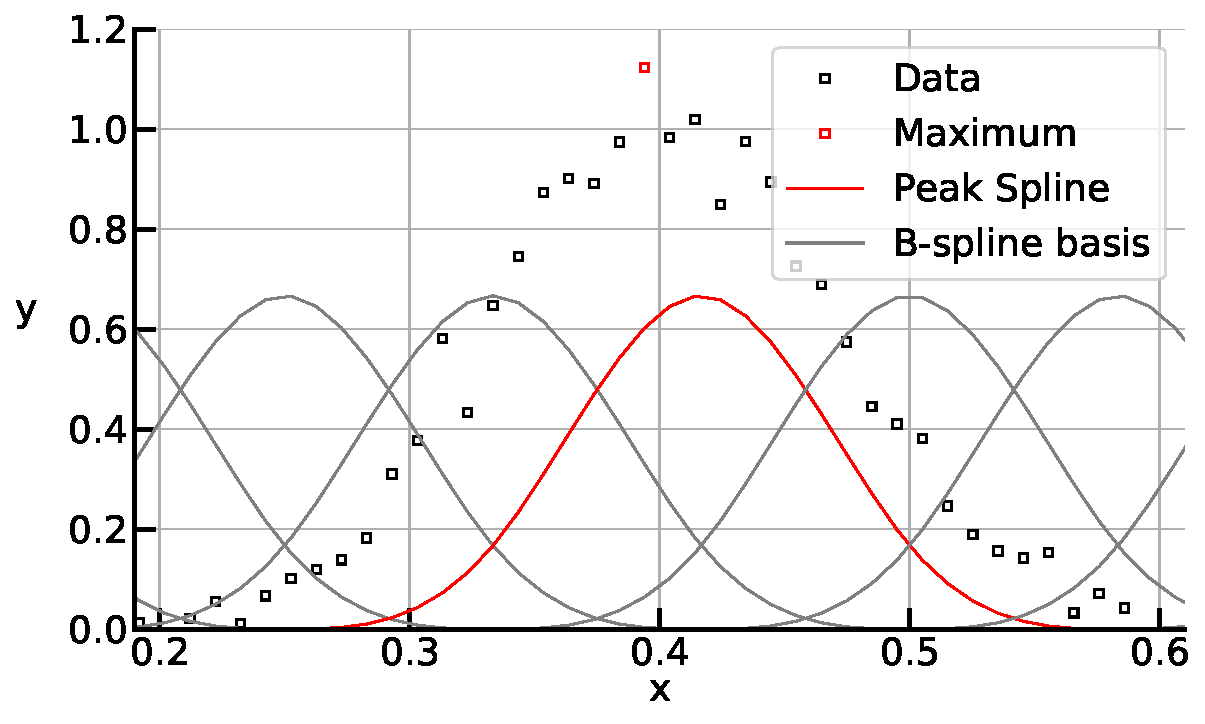
\includegraphics[width=\linewidth]{../thesisplots/peak_spline.pdf}
	\caption{Identification of the peak spline based on data}
	\label{fig:peak_spline}
\end{figure}


The corresponding matrix for $k$ splines is given as 

\begin{align}\label{eq:D_c_unimodal}
	\vec{D}_c^{unimodal} = \begin{pmatrix} -1 & 1 \\ 
		& \ddots & \ddots  \\
		& & -1 & 1
	\end{pmatrix} \in \mathbb{R}^{k-1 \times k}
\end{align}

The weights $v_j$ to incorporate the peak constraint have the following structure, i.e.

\begin{align}\label{eq:v_peak_1}
	v_j(\vec{\beta}) &= \begin{cases} 
		0, \quad \text{if} \ \Delta^1\beta_j \ge 0 \\ 
		1, \quad \text{if} \ \Delta^1\beta_j  < 0.
	\end{cases}, \quad \text{for} \ j=2, \dots, j_{peak}-1
\end{align}

and

\begin{align}\label{eq:v_peak_2}
	v_j(\vec{\beta}) &= \begin{cases} 
		0, \quad \text{if} \ \Delta^1\beta_j \le 0 \\ 
		1, \quad \text{if} \ \Delta^1\beta_j > 0.
	\end{cases}, \quad \text{for} \ j=j_{peak}+1, \dots, k.
\end{align}

The weight $v_{j_{peak}}$ for the \emph{peak spline} is given by $v_{j_{peak}}(\vec{\beta}) = 0$. 

When assuming a valley in the data, the same approach as above can easily be used by multiplying the data with $-1$ or by always doing the inverse operation, i.e. finding the index $j_{valley}$ of the \emph{valley spline}, then constraining all splines for $j < j_{valley}$ to be monotonic decreasing, i.e. $\Delta^1 \beta_j \le 0$ for $j = 1, \dots, j_{valley}-1$, and all splines for $j > j_{valley}$ to be monotonic increasing, i.e. $\Delta^1 \beta_j \ge 0$ for $j = j_{valley}+1, \dots, k$. The coefficient $\beta_{j_{valley}}$ stays unconstrained. 

The weights $v_j$ to consider a valley constraint are given by

\begin{align}\label{eq:v_valley_1}
	v_j(\vec{\beta}) &= \begin{cases} 
		0, \quad \text{if} \ \Delta^1\beta_j \le 0 \\ 
		1, \quad \text{if} \ \Delta^1\beta_j > 0
	\end{cases}, \quad \text{for} \ j=2, \dots, j_{valley}-1
\end{align}

and 

\begin{align}\label{eq:v_valley_2}
	v_j(\vec{\beta}) &= \begin{cases} 
		0, \quad \text{if} \ \Delta^1\beta_j \ge 0 \\ 
		1, \quad \text{if} \ \Delta^1\beta_j < 0.
	\end{cases}, \quad \text{for} \  j=j_{valley}+1, \dots, k.
\end{align}

The weight $v_{j_{valley}}$ for the \emph{valley spline} is given by $v_{j_{valley}}(\vec{\beta}) = 0$.

%%%%%%%%%%%%%%%%%%%%%%%%%%%%%%%%%%%%%%%%%%%%%%%%%%%%%%%%%%%%%%%%%%%%%%%%%%%%%%%%%%%%%%%%%%%%%%%%%%%%%%%%%%%%%%%%
\subsection{Boundedness Constraint}

For certain physical systems, it is known a priori that the measured quantity cannot be smaller than zero, i.e. $f(x) \ge 0$. Using data-driven modeling on noisy data can lead to predictions in the interpolation and extrapolation regime, which may not hold this constraint due to uncertainties captured by the data. It is therefore appropriate to apply the user-defined constraint of boundedness from below.

The user-defined constraint for boundedness from below by $M=0$ uses as mapping matrix $\vec{D}_c$ the B-spline basis matrix $\vec{X} \in \mathbb{R}^{n \times k}$. The weighting matrix $\vec{V} \in \mathbb{R}^{n\times n}$, with individual weights $v_j$, is specified as follows:

\begin{align} \label{eq:v_boundedness}
	v_j(\vec{\beta}) = \begin{cases} 
		0, \quad \text{if} \ f(x^{(j)}) \ge M\\ 
		1, \quad \text{if} \ f(x^{(j)})  < M 		
	\end{cases} \text{for} \ j=1, \dots, n.
\end{align}

Using different values of $M$ allows us to bound from below from any number $M$. Switching the comparison operators in (\ref{eq:v_boundedness}) enables us to bound functions from above. 

%%%%%%%%%%%%%%%%%%%%%%%%%%%%%%%%%%%%%%%%%%%%%%%%%%%%%%%%%%%%%%%%%%%%%%%%%%%%%%%%%%%%%%%%%%%%%%%%%%%%%%%%%%%%%%%%
\subsection{Jamming Constraint}

Jamming the function $f(x)$ by some point $p = \{x^{(jamm)}, y^{(jamm)}\}$ means that the estimated function $f(x^{(jamm)}) \approx y^{(jamm)}$. This can be incorporated using the B-spline basis matrix $\vec{X} \in \mathbb{R}^{n \times k}$ as mapping matrix $\vec{D}_c$ and a weighting matrix $\vec{V} \in \mathbb{R}^{n \times n}$ given by

\begin{align} \label{eq:v_jamming}
	v_j(\vec{\beta}) = 
		\begin{cases}
			0, \quad \text{if} \ x^{(j)} \ne x^{(jamm)} \\
			1, \quad \text{if} \ x^{(j)} = x^{(jamm)} 
	\end{cases} \text{for} \ j = 1, \dots, n.
\end{align} 


%%%%%%%%%%%%%%%%%%%%%%%%%%%%%%%%%%%%%%%%%%%%%%%%%%%%%%%%%%%%%%%%%%%%%%%%%%%%%%%%%%%%%%%%%%%%%%%%%%%%%%%%%%%%%%%%%
%%%%%%%%%%%%%%%%%%%%%%%%%%%%%%%%%%%%%%%%%%%%%%%%%%%%%%%%%%%%%%%%%%%%%%%%%%%%%%%%%%%%%%%%%%%%%%%%%%%%%%%%%%%%%%%%%
\section{n-d Constraint Function Estimation}

The extension from one input to multiple input dimensions uses the concept of additive models given in Chapter \emph{Additive Models}. Given input data $\{ x_1^{(i)}, \dots, x_p^{(i)}, y^{(i)}\}$ for $i = 1, \dots, n$ and $p$ as the number of inputs, the combined model using all available B-splines and tensor-product splines is given as

\begin{align} \label{eq:tps_all}
	y = f(x_1,..., x_p) = \sum_{j=1}^p s_j(x_j) + \sum_{j=1}^{p-1} \sum_{l>j}^p t_{j, l}(x_j, x_l)
\end{align}

where $s_j(x_j)$ is the B-spline estimate given by $s_j(x_j) = \vec{X}_j \vec{\beta}_j$ and $t_{l, j}(x_l,x_j)$ is the tensor-product estimate is given by $t_{j, l}(x_j,x_l) = \vec{X}_{j, l} \vec{\beta}_{j, l}$. The number of individual estimates is given by 

\begin{align}
	n_{total} = p + \frac{p(p-1)}{2}.  
\end{align}


The constrained penalized least squares objective function for additive models can now be written similar to (\ref{eq:OF_3}) as

\begin{align}\label{eq:OF_6}
	Q_6(\vec{y}, \vec{\beta}) = Q_1(\vec{y}, \vec{\beta}) + \transpose{\vec{\lambda}}_s	\vec{\mathcal{J}}_s(\vec{\beta}; \vec{d}) + \transpose{\vec{\lambda}}_c \vec{\mathcal{J}}_c(\vec{\beta}; \vec{c}).
\end{align}

with $\vec{\lambda}_s \in \mathbb{R}^{n_{total}}$ and  $\vec{\lambda}_c \in \mathbb{R}^{n_{total}}$  defined as vectors with one value of smoothness and constraint parameter for each estimate, respectively. 

The objective function (\ref{eq:OF_6}) is then optimized, i.e.

\begin{align}\label{eq:optimization_problem_6}
	\vec{\hat \beta}_{PLS,c,nd} = \arg \min_{\vec{\beta}} Q_5(\vec{y}, \vec{\beta}),
\end{align}

using the penalized iteratively reweighted least squares algorithm to obtain the coefficients $\vec{\hat{\beta}}_{PLS,c,nd}$. 

We now need to specify the three parts of the objective function in (\ref{eq:OF_6}). 

%%%%%%%%%%%%%%%%%%%%%%%%%%%%%%%%%%%%%%%%%%%%%%%%%%%%%%%%%%%%%%%%%%%%%%%%%%%%%%%%%%%%%%%%%%%%%%%%%%%%%%%%%%%%%%%%%
\subsection{Data Term}



Assuming the use of $k$ splines for the B-spline estimates and $k^2$ splines for the tensor-product estimates, the total number of coefficients to be determined is given by 

\begin{align}\label{eq:tps_total_number_of_coef}
	k_{total} = pk + \frac{p(p-1)}{2}k^2. 
\end{align}

Since all B-spline and tensor-product spline models follow a linear model structure, we can combine them into one large model given by

\begin{align}\label{eq:tps_lin_mod}
	\vec{y} = \vec{X} \vec{\beta}
\end{align}

where the matrix $\vec{X} \in \mathbb{R}^{n \times k_{total}}$ is given by a horizontal concatenation of the individual bases and the combined coefficient vector $\vec{\beta} \in \mathbb{R}^{k_{total}}$ is given by a vertical concatenation of the individual coefficient vectors. The model has then the following form

\begin{align}\label{eq:tps_lin_model_verbose}
	\vec{y} = \vec{X} \vec{\beta} = 
	\begin{pmatrix} \vec{X}_{s_1} \dots \vec{X}_{s_p} \ \vec{X}_{t_{1,2}} \dots \vec{X}_{t_{p-1,p}} \end{pmatrix} 
	\begin{pmatrix} \vec{\beta}_{s_1} \\ 
		\vdots  \\ 
		\vec{\beta}_{s_p} \\ 
		\vec{\beta}_{t_{1,2}} \\ 
		\vdots \\ 
		\vec{\beta}_{t_{p-1,p}} \\
	\end{pmatrix}.
\end{align}

The data term $Q_1(\vec{y}, \vec{\beta})$ in the constrained penalized least squares objective function given in (\ref{eq:OF_6}) can now be evaluated using arbitrary input dimensions. 

%%%%%%%%%%%%%%%%%%%%%%%%%%%%%%%%%%%%%%%%%%%%%%%%%%%%%%%%%%%%%%%%%%%%%%%%%%%%%%%%%%%%%%%%%%%%%%%%%%%%%%%%%%%%%%%%%
\subsection{Smoothness Term}

The combined smoothness penalty term $\vec{\mathcal{J}}_s(\vec{\beta}; \vec{d}) \in \mathbb{R}^{n_{total}}$ is then given as

\begin{align}\label{eq:J_s_ndim}
	\vec{\mathcal{J}}_s(\vec{\beta}; \vec{d}) &= 
	\begin{pmatrix}
		\mathcal J_{s_1}(\vec{\beta}_{s_1}; d_{s_1}) \\ 
		\vdots \\ 
		\mathcal J_{s_p}(\vec{\beta}_{s_p}; d_{s_p}) \\
		\mathcal J_{t_{1,2}}(\vec{\beta}_{t_{1,2}}; d_{t_{1,2}}) \\
		\vdots \\
		\mathcal J_{t_{p-1,p}}(\vec{\beta}_{t_{p-1,p}}; d_{t_{p-1,p}}) \\
	\end{pmatrix}
\end{align}

with $\mathcal J_e(\vec{\beta}_e; d_e) = \transpose{\vec{\beta}}_e \transpose{\vec{D}}_{d_e} \vec{D}_{d_e} \vec{\beta}_e$ determining the smoothness penalty term using the coefficients $\vec{\beta}_e$ and mapping matrix $\vec{D}_{d_e}$ for each estimate $e$ for $e=s_1, \dots, s_p, t_{1,2}, \dots, t_{p-1,p}$. The vector $\vec{d} \in \mathbb{R}^{n_{total}}$ consists of the orders $d_e$ determining the mapping matrix $\vec{D}_{d_e}$ of the smoothness constraint for each individual estimate $e$. 

%%%%%%%%%%%%%%%%%%%%%%%%%%%%%%%%%%%%%%%%%%%%%%%%%%%%%%%%%%%%%%%%%%%%%%%%%%%%%%%%%%%%%%%%%%%%%%%%%%%%%%%%%%%%%%%%%
\subsection{Constraint Term}
The combined constraint penalty term $\vec{\mathcal{J}}_c(\vec{\beta}; \vec{c}) \in \mathbb{R}^{n_{total}}$ is then given as

\begin{align}\label{eq:J_c_ndim}
	\vec{\mathcal{J}}_c(\vec{\beta}; \vec{c}) &= 
	\begin{pmatrix}
		\mathcal J_{s_1}(\vec{\beta}_{s_1}; c_{s_1}) \\ 
		\vdots \\ 
		\mathcal J_{s_p}(\vec{\beta}_{s_p}; c_{s_p}) \\
		\mathcal J_{t_{1,2}}(\vec{\beta}_{t_{1,2}}; c_{t_{1,2}}) \\
		\vdots \\
		\mathcal J_{t_{p-1,p}}(\vec{\beta}_{t_{p-1,p}}; c_{t_{p-1,p}}) \\
	\end{pmatrix}
\end{align}

with $\mathcal J_e(\vec{\beta}_e; c_e) = \transpose{\vec{\beta}}_e \transpose{\vec{D}}_{c_e} \vec{V}_e \vec{D}_{c_e} \vec{\beta}_e$ determining the constraint penalty term using the coefficients $\vec{\beta}_e$, the mapping matrix $\vec{D}_{c_e}$ and the weighting matrix $\vec{V}_e$ for each estimate $e$ for $e=s_1, \dots, s_p, t_{1,2}, \dots, t_{p-1,p}$. The vector $\vec{c} \in \mathbb{R}^{n_{total}}$ consists of the constraint type $c_e$, e.g. monoton increasing, determining the mapping matrix $\vec{D}_{c_e}$ for each individual estimate $e$. 


%%%%%%%%%%%%%%%%%%%%%%%%%%%%%%%%%%%%%%%%%%%%%%%%%%%%%%%%%%%%%%%%%%%%%%%%%%%%%%%%%%%%%%%%%%%%%%%%%%%%%%%%%%%%%%%%%%%%
\subsection{Mapping Matrices for Tensor-Product Splines}

The tensor-product spline basis is given by the Kronecker product of two B-spline bases, as depicted in Chapter \emph{Tensor-product splines}. To extend the framework of mapping matrices to two dimensions and tensor-product splines, we again use the concept of Kronecker products. 

We want to penalize adjacent coefficient differences to enforce smoothness, but this time, in two dimensions. Therefore, an appropriate spatial neighbourhood needs to be defined. An example for such neighbourhood for the coefficient $\beta_{j, k}$ is given by the coefficients left and right, i.e. $\beta_{j-1, k}$ and $\beta_{j+1, k}$, and the coefficients above and below, i.e. $\beta_{j, k-1}$ and $\beta_{j,k+1}$. 

Let us now define the mapping matrices $\vec{D}_{d_1}$ and $\vec{D}_{d_2}$ of orders $d_1$ and $d_2$ for each dimension, respectively. Using the Kronecker product, we generate the expanded mapping matrix $\vec{D}_{d_{1}, exp} = \vec{I}_{d_2} \otimes \vec{D}_{d_1}$ with the identity matrix $\vec{I}_{d_2} \in \mathbb{R}^{d_2 \times d_2}$ and $\vec{D}_{d_2,exp} = \vec{D}_{d_2} \otimes \vec{I}_{d_1}$ with the identity matrix $\vec{I}_{d_1} \in \mathbb{R}^{d_1 \times d_1}$. 

Row-wise mappings of order $d_1$ and column-wise mappings of order $d_2$ are now obtained by applying the expanded difference matrix $\vec{D}_{d_1,exp}$ and $\vec{D}_{d_2,exp}$ to the coefficient vector $\vec{\beta}$, respectively. 

Using these concepts, in principle every possible pair of one dimensional user-defined constraints can now be constructed, e.g. unimodality in two dimensions would be obtained using the unimodal penalty matrix depicted above for each dimension. 

The penalty term for the constraint given by $c_1$ for dimension $1$ and $c_2$ for dimension $2$ then has the form

\begin{align} \label{eq:J_c_tps}
	\mathcal J_c(\vec{\beta}; c_1, c_2) = \transpose{\vec{\beta}} \transpose{\vec{D}}_{c_1,exp} \vec{V}_1 \vec{D}_{c_1,exp} \vec{\beta} + \transpose{\vec{\beta}} \transpose{\vec{D}}_{c_2,exp} \vec{V}_2 \vec{D}_{c_2,exp} \vec{\beta}
\end{align}

with $\vec{D}_{c_1,exp} = \vec{I}_{d_2} \otimes \vec{D}_{c_1}$ and $\vec{D}_{c_2,exp} = \vec{D}_{c_2} \otimes \vec{I}_{d_1}$ as individual mapping matrices  and the weighting matrices $\vec{V}_1$ and $\vec{V}_2$ according to the given constraints.

The constrained penalized least squares objective function in (\ref{eq:OF_6}) can now be used to estimate the coefficients $\vec{\beta}_{PLS,c, nd}$. \cite{fahrmeir2013regression}

%%%%%%%%%%%%%%%%%%%%%%%%%%%%%%%%%%%%%%%%%%%%%%%%%%%%%%%%%%%%%%%%%%%%%%%%%%%%%%%%%%%%%%%%%%%%%%%%%%%%%%%%%%%%%%%%%%%
\subsection{2-d Example}

As example for the n-d constraint function estimation, we take a look at the function 

\begin{align} \label{eq:2d_test_func}
	f(x_1, x_2) = 2\exp{\Big(-\frac{(x_1 - 0.25)^2}{0.08}\Big)} + x_2^2 + \eta
\end{align}

for $x_1 \in [0,1]$ and $x_2 \in [0,1]$ and random Gaussian noise $\eta$ with $\sigma_{noise} = 0.1$. Therefore we expect a peak in dimension $x_1$ as well as increasing behavior for dimension $x_2$, see Figure \ref{fig:2d_example}. The user-defined constraints are therefore $c_1 = \text{unimodal}$ and $c_2 = \text{monotonic increasing}$ Using this knowledge, we create a model with the following characteristics:

\begin{itemize}
	\item B-spline smooth $s_1(x_1)$: $k_{x_1} = 50$, $c = c_1$, $\lambda_s = 1$ and $\lambda_c = 6000$
	\item B-spline smooth $s_2(x_2)$: $k_{x_2} = 50$, $c = c_2$, $\lambda_s = 1$ and $\lambda_c = 6000$
\end{itemize}

The fit for this model as well as the individual estimates $s_1(x_1)$ and $s_2(x_2)$ are shown in Figure \ref{fig:2d_example}. The model fits the data quite well and holds the specified constraints for the individual dimensions.

\begin{figure}[H]
	\centering
	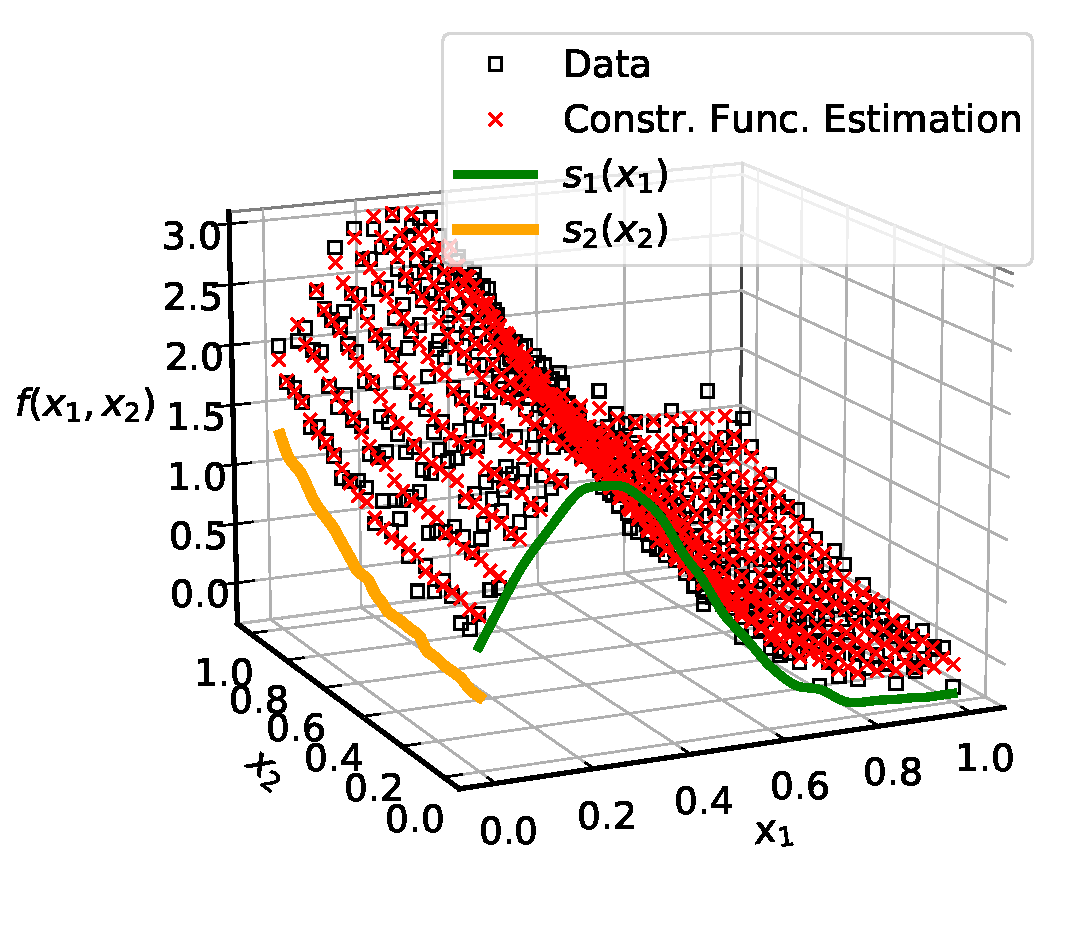
\includegraphics[width=\linewidth]{../thesisplots/2d_example.pdf}
	\caption{2-d test function for n-d constrained function estimation}
	\label{fig:2d_example}
\end{figure}



\printbibliography

\end{document}